%
% Szakdolgozatminta az Eszterházy Károly Katolikus Egyetem
% matematika illetve informatika szakos hallgatóinak.
%

\documentclass[
% opciók nélkül: egyoldalas nyomtatás, elektronikus verzió
% twoside,     % kétoldalas nyomtatás
% tocnopagenum,% oldalszámozás a tartalomjegyzék után kezdődik
]{thesis-ekf}

\usepackage[T1]{fontenc}
\PassOptionsToPackage{defaults=hu-min}{magyar.ldf}
\usepackage[magyar]{babel}
\usepackage{mathtools,amssymb,amsthm,pdfpages}
\footnotestyle{rule=fourth}

\newtheorem{tetel}{Tétel}[chapter]
\theoremstyle{definition}
\newtheorem{definicio}[tetel]{Definíció}
\theoremstyle{remark}
\newtheorem{megjegyzes}[tetel]{Megjegyzés}

\definecolor{lgreen}{rgb}{.90, .90, .96}
\definecolor{dkgreen}{rgb}{0,.6,0}
\usepackage{listings,xcolor,caption}
\lstset{
  basicstyle=\footnotesize,
  numbers=left,
  breaklines,
  postbreak=\hbox{$\color{blue}\hookrightarrow\ $},
  xleftmargin=2cm,
  xrightmargin=2cm,
  backgroundcolor=\color{lgreen},
  frame=tlbr,
  framesep=3pt,
  inputencoding=utf8/latin2,
  language        = php,
  basicstyle      = \small\ttfamily,
  keywordstyle    = \color{blue},
  stringstyle     = \color{red},
  identifierstyle = \color{dkgreen},
  commentstyle    = \color{gray},
  emph            =[1]{php},
  emphstyle       =[1]\color{black},
}
\renewcommand{\lstlistingname}{Programkód}

\begin{document}
	\institute{Matematikai és Informatikai Intézet}
	\title{Webes vizsgáztató rendszer}
	\author{Kecse Károly Dániel\\Programtervező informatikus}
	\supervisor{Dr. Király Roland\\egyetemi docens}
	\city{Eger}
	\date{2023}
	\maketitle
	\tableofcontents
	
	\chapter*{Bevezetés}
	\addcontentsline{toc}{chapter}{Bevezetés}
	A szakdolgozat célja, hogy egy olyan rendszert biztosítsak az iskoláknak, amivel lehetőséget adok a tanároknak, hogy egy helyen tárolják az órákhoz létrehozott tananyagot az ezekhez kapcsolódó számonkérési és gyakorlási lehetőségekkel együtt, amiknek a kitöltésére egy jól szabályozható felületet biztosítunk a diákoknak.
 
	Egy másik elvárásom az volt, hogy a szoftvert tetszőleges eszközön lehessen használni úgy, hogy a megjelenítés minden esetben komfortos legyen és ne érezzük kényelmetlen egyetlen funkciónak a használatát sem, legyen az akár egy kisebb kijelzőjű mobil vagy egy szélesebb monitor. Így a választásom a webes megjelenítésre esett, aminek egyetlen feltétele a megfelelő működéshez, hogy stabil internet hozzáféréssel rendelkezzünk.

        A fenti elvárásoknak megfelelően megszületett a \emph{webes vizsgáztató rendszer}, amely egy olyan webes alkalmazás, amelyben lehetőségünk van arra, hogy csoportokat kezeljünk, esetlegesen annak tagjaival csevegjünk, vagy kurzusokon vegyünk részt. A bejelentkezést követően egy olyan főoldal (\ref{fig-index-page}.~ábra) fogad minket, amely kilistázza az elérhető kurzusainkat illetve csoportjainkat.
        \begin{figure}[ht!]
    	\centering
    	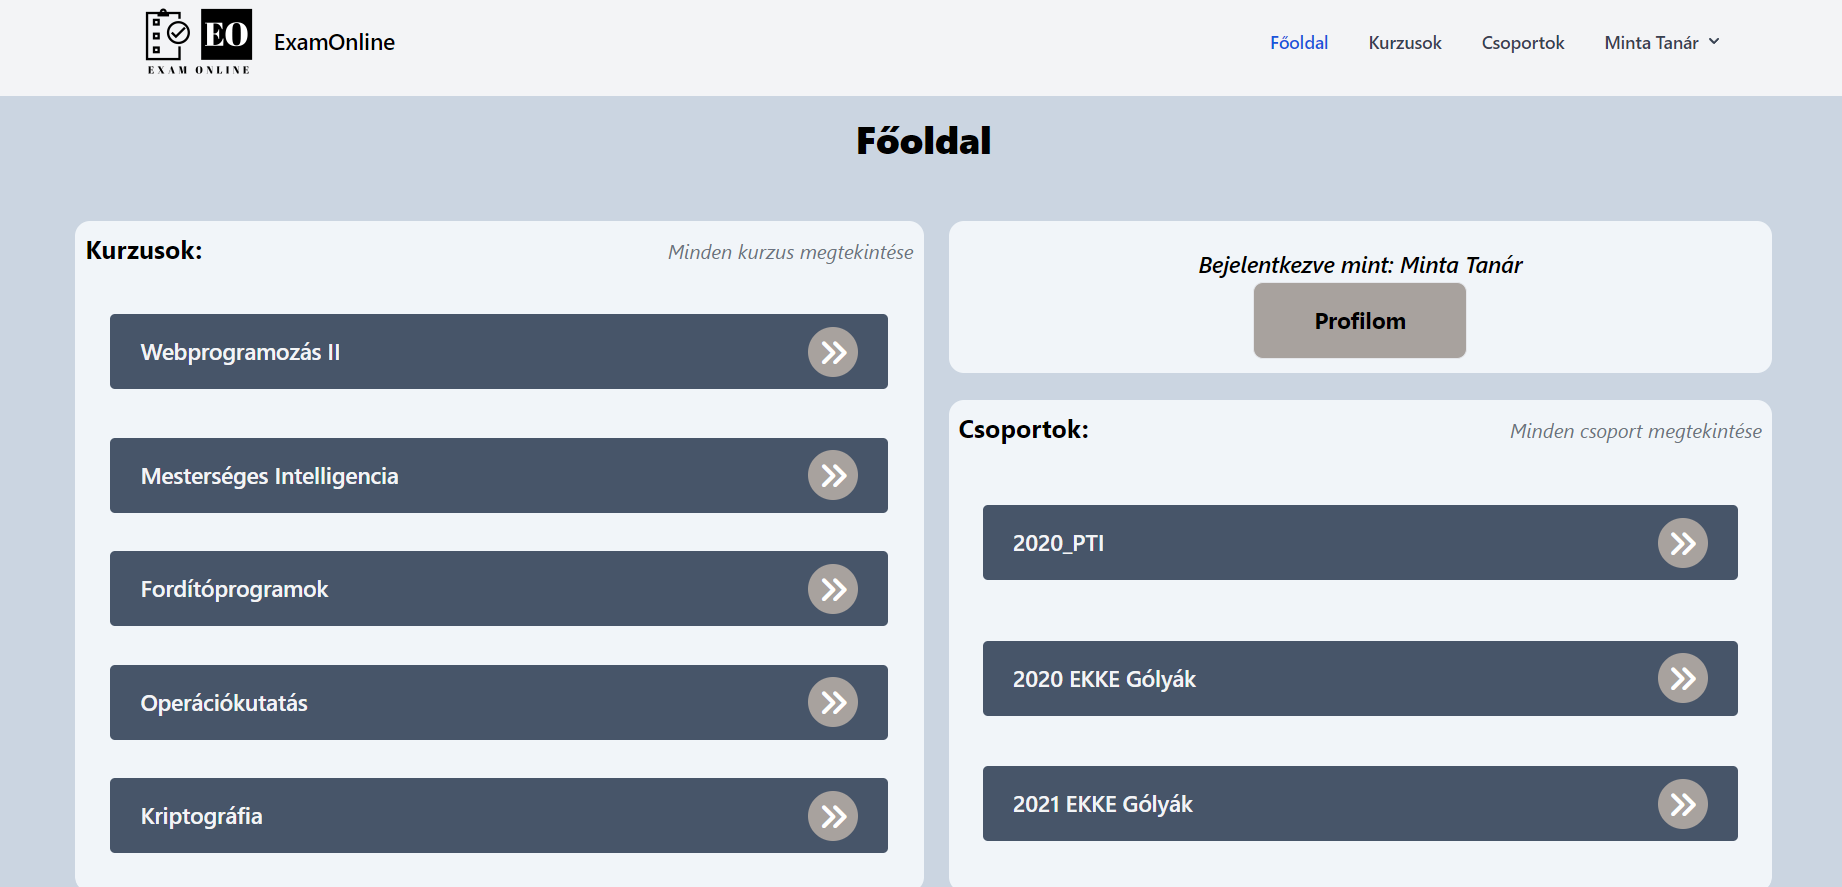
\includegraphics[width=15cm]{index_page.png}
            \caption{Bejelentkezést követő főoldal}
    	\label{fig-index-page}
        \end{figure}

        A projekt egyik fő részét a csoportok képzik. Itt nincsen semmilyen korlátozás arra, hogy ki hozhat létre, kezelhet csoportokat. Egyetlen megkötés, hogy az adott csoporthoz való műveletek (frissítés és törlés) csak az azt létrehozó felhasználónak vannak biztosítva. A csoportok bemutatásáról, funckióiról és képernyőképeiről részletesebb leírást \az{\ref{Csoportok-bemutat}}.~fejezetben olvashatnak.

        A rendszer másik, legnagyobb és legjelentősebb egységét a kurzusok jelentik. Ezek segítségével tudtam tananyagokat és teszteket készíteni a különböző tantárgyakhoz. Ennek az egységnek a működése nagyban függ attól, hogy milyen a bejelentkezett felhasználónak a jogosultsági köre. 
        
        Amennyiben tanárok vagyunk, lehetőségünk nyílik arra, hogy kurzusokat készítsünk, ahol tananyagokat illetve teszteket hozhatunk létre. Megszabhatjuk, hogy mely csoportok és milyen diákok érhetik el az itt található tartalmakat, illetve milyen időintervallumban férhetnek hozzá bizonyos feladatsorokhoz. 
        
        Tanulóként megtekinthetjük a kurzus tananyagát, kitölthetjük a teszteket, viszont a vizsgák kitöltésének eredményei közül csak a sajátunkat láthatjuk. 
        
        Ezzel ellentétben a tanár megtekintheti a kurzus minden tagjának az eredményét. Akár azt is megteheti, hogy bizonyos próbálkozásokat töröl, ilyenkor növelve a lehetséges kitöltések számát az adott diáknak. A kurzusokról később bővebben \az{\ref{Kurzusok-bemutat}}.~fejezetben fogok írni. Az ezekhez tartozó különböző tesztekről (felépítés, működés, különbségek) \az{\ref{Tesztek-bemutat}}.~fejezetben olvashatnak.

        Egy harmadik, kisebb, ám annál jelentősebb funkció a tanárok regisztrálása. Mivel a navigációs sávban mindenki által elérhető regisztrációs felülettel csak tanulóként regisztrálhatunk, szükségessé vált az, hogy legyen egy olyan jogosultsági kör, aminek egyetlen feladata a tanárok felvitele a rendszerbe. Ez az admin felhasználó lesz (akit a Seeder segítségével adhatunk az adatbázishoz), akinek a ,,Kurzusok'' és ,,Csoportok'' helyett egy ,,Tanár hozzáadása'' menüpont lesz látható a bejelentkezés után, amely segítségével oktatókat vihet fel a rendszerbe.

        A szakdolgozat további részében megtalálható azoknak az alkalmazásoknak az elemzése, amelyek alapján született az alap elképzelés a rendszerről (\ref{kokurensek-label}.~fejezet). 
        
        Ezt követően az adatbázis felépítését fogom tárgyalni \az{\ref{Adatbazis}}.~fejezetben, ahol a két fő egység elkészítéséhez szükséges táblákat, illetve azok szükségességét fogom taglalni.

        Ezek után felvezetem \az{\ref{Technologiak-bemutat}}.~fejezetben azokat a fontosabb keretrendszereket és technológiákat, amelyek nagyban hozzájárultak a projekt elkészítésében. Az itt tárgyalt Laravel és Livewire keretrendszerekről \az{\ref{Laravel-mukodes}}.~és \az{\ref{Livewire}}.~fejezetben fogok részletesebben írni, ahol a felhasznált elemek működési elvét ismertetem példakódok segítségével.

        \Az{\ref{Kulso}}.~fejezetben a külső komponensekről fogok említést tenni, amiben különböző csomagok, könyvtárak és tesztelési környezetek leírásáról olvashatnak.
	
	\chapter{A hasonló alkalmazásokról}\label{kokurensek-label}
	A fejezetben összegyűjtöttem azokat az alkalmazásokat, amiket a témakörben relevánsnak ítéltem meg. Ezek közül a legtöbbhöz volt szerencsém eddigi tanulmányaim alatt, ezért van némi tapasztalatom is velük. Az alábbi rendszerek tüzetesebb elemzése után igyekeztem kigyűjteni azokat a funkciókat, amikkel kapcsolatban pozitív volt az élményem illetve elengedhetetlennek ítéltem meg.
	
	\section{Alternatívák és jellemzők, észrevételek}
	\subsection{Moodle}
	Az Egyetem elearning rendszerét\cite{Moodle} használtuk a legtöbb órán, ezért erről van az egyik legjobban kirajzolódott véleményem. A projektemben belüli kurzusok felépítése ehhez a rendszerhez hasonlít, hiszen kifejezetten tetszett, hogy a számonkérés és a tananyagnak az elérése egy egységes rendszerben elérhető. Ennek a rendszernek talán két dolgot lehetne felróni: rengeteg olyan felesleges információt tár elénk az oldal, amelyet valószínűleg soha nem fogunk használni, ez pedig meglehetősen csökkenti a felület átláthatóságát. A másik, ettől sokkal kisebb probléma, hogy a számonkéréseknek a feladattípusai számomra eléggé egyhangúak.
	
	\subsection{Pegazus}
	A Pegazus\cite{Pegazus} egy általunk kevéssé használt alkalmazás, így sajnos csak minimális személyes tapasztalatom van vele kapcsolatban, éppen ezért hallgató társaimtól is érdeklődtem, hogy milyen véleményük van a használatával kapcsolatban. Az első dolog, amit észrevettem, hogy a moodle-höz képest rendkívül letisztult és szép megjelenéssel rendelkezik az oldal. Emellett nagyon sokféle feladattípus közül lehet választani, ami nagy előny. A másik pozitívum, hogy itt is elérhető a kurzusokhoz tartozó tananyag a számonkéréssel együtt (bár azt hallottam, hogy a tesztek használata nem túl elterjedt a rendszeren belül). Az én célom egy ehhez hasonló rendszer kialakítása volt, amely gyorsabb oldalelérést tesz lehetővé, és amely a diákok számára lehetővé teszi, hogy közelebb érezzék magukat egymáshoz a használat során.
	
	\subsection{Redmenta}
	A Redmenta\cite{Redmenta} egy olyan webes alkalmazás, amely a Pegazus sokszínű feladattípus kínálatával vetélkedik, így biztosítva egy elképesztően változatos vizsgázási élményt. Felhasználási köre leginkább az általános és középiskolák körében elterjedt, viszont volt már rá példa, hogy itt, az Egyetemen is ezt alkalmaztuk egy online vizsga keretén belül. Egyedül tesztek készítésére és kitöltésére használható, ezért a Redmenta tudása számomra kissé korlátozott.
	
	\subsection{Quizizz}
	A Quizizz\cite{Quizizz} egy olyan alkalmazás, amelyet leginkább kvízek írására fejlesztettek ki, és hasonlóan a Redmentához, lehetővé teszi a tesztek készítését. A Quizizz különböző animációkkal, effektekkel, játékos elemekkel próbálja szórakoztatóvá tenni a tanulást, ezért is elterjedtebb általános iskolák körében. Sajnos a legtöbb funkció előfizetéshez kötött, így az alkalmazásban való tevékenységünk kissé korlátozottabb lehet, mint például a Redmenta vagy a Pegazus esetében.
	
	\section{Következtetések}
	A fentiekben felsoroltak alapján felállítottam néhány elvárást, amiknek a szem előtt tartásával terveztem meg és implementáltam a projekt egyes funkcióit. Ezek az alábbiak, amiknek a leírásáról a többi fejezetben esik majd szó:
	\begin{itemize}
		\item Letisztult, felhasználó barát felület (mobilra is)
		\item Tananyag elérése a számonkéréssel együtt egy rendszerben
		\item Változatos feladattípusok (jelenleg 4 típus)
		\item Gyakorlási lehetőség biztosítása az egyes órákhoz
		\item Olyan funkciók készítése és megjelenítése, amelyeket én is szívesen látnék, mint diák
	\end{itemize}
	Sajnos a fentiekben felsorolt alkalmazásokhoz képest ez a projekt eléggé gyerekcipőben jár, viszont ezeknek a jól bevált módszereit igyekeztem úgy implementálni, hogyha nem is módosítás nélkül, de minimális átdolgozással problémamentesen bővíthető legyen. Ilyen például több feladattípus felvitele, tananyaghoz fájlok feltöltésének biztosítása, statisztikák lekérdezése a megadott válaszoknak megfelelően.
	
	
	\chapter{Felhasznált technológiák}\label{Technologiak-bemutat}
	   \section{Laravel}
	       A Laravel\cite{LaravelMVC} egy PHP nyelvhez készített nyílt forráskódú,  ingyenes backend keretrendszer, amely MVC tervezési mintát használ.
            Ez annyit tesz, hogy a rendszerünk működése 3 rétegre van felosztva:
            \begin{itemize}
                \item \textbf{M}odel: Osztályok használatával biztosít adatbázison végezhető műveleteket metódushívásokon keresztül.
                \item \textbf{V}iew: Egy olyan nézet, ahol általában a kontrollerből érkező adatokat jelenítjük meg. Az oldalon biztosíthatunk a felhasználónak navigációs lehetőségeket különböző útvonalak használatával, amelyek egy-egy Controller függvényét hívják meg.
                \item \textbf{C}ontroller: A View és a Model között biztosít összeköttetést. Az oldalakról esetlegesen érkező adatok segítségével végezhet műveleteket egy adott modellen, vagy a megjelenítendő oldalnak előállíthatja a szükséges adatokat. Egy kontrollerben lefutott utasítássorozat után vagy visszaad egy nézetet az összeállított adatokkal együtt, vagy átnavigál minket egy másik útvonalra.
                
            \end{itemize}
            A Laravel egyik legnagyobb előnye a számomra, hogy rendkívül jól dokumentált, így nem jelentett különösebb problémát a felmerülő hibák megoldását megtalálni, illetve eddig ismeretlen lehetőségek után keresgélni (például Queued Job, Broadcast). Folyamatosan fejlesztik, hiszen 2023 februárjában került kiadásra a Laravel 10-es verziója (még ha az eddigi egyik legkisebb frissítés is). Egyszerű módszerrel biztosítja az egyes útvonalak (route-ok) kezelését különböző HTTP kérési típusok megkülönböztetésével együtt. Másik pozitívuma, hogy a felhasználói autentikációhoz is van rengeteg már elkészített és megfelelően integrált megoldás, így sem a bejelentkezést, sem a munkamenet-kezelést nem kell az alapjaitól kezdve megvalósítanunk.
            
            A Laravel alapból érkezik egy Artisan-nal, ami egy CLI (Parancssori Felhasználói Felület). Ennek segítségével a projektünkben generálhatunk fájlokat (Migration, Model, Controller, Resource, Job, Policy), lefuttathatjuk a megírt Migration fájljainkat illetve a projektnek a szerveren való futtatását is elvégzi.
	
	   \section{Livewire}
            Szerettem volna egy olyan frontend-kezelő keretrendszert használni, amihez nem kell több hónapos tapasztalat ahhoz, hogy bonyolultabb feladatokat is viszonylag gyorsan és hatékonyan tudjak implementálni, illetve könnyedén tudjam a Laravel-es projekten belül használni. Ígya választásom a Livewire-re\cite{LaravelLivewire} esett, ami egy kifejezetten Laravel-hez írt fullstack keretrendszer. Egyszerűvé teszi a dinamikus felületek létrehozását, az összetettebb űrlapkezelést -- mindezt úgy, hogy közben maradhatunk a jól megszokott Laravel szintaxisoknál. 
        
            Az ilyen módon készített fájlok sem különböznek túlságosan az egyszerű Laraveles működéstől: egy LiveWire komponens létrehozása során kapunk egy külön Livewire Controller-t illetve egy Blade fájlt, amelyek szoros kapcsolatban állnak egymással. A használatához ezt kell majd beimportálnunk azokon az oldalakon, ahol szeretnénk a már kész komponenseinket használni. 
            
            Ilyen technikával készültek a projekt tesztjeinek létrehozását, szerkesztését, kitöltését, valamint a csoportok és felhasználók keresését biztosító elemek. Egyszerű asszociatív tömbökkel tudunk dolgozni, amiknek az értékeit hozzárendelhetjük az űrlapunk egyes beviteli mezőinek értékéhez. 
            
            A backend és frontend kommunikációja a ,,\emph{render()}'' metóduson keresztül biztosított, amit az oldalak betöltésénél illetve minden, a komponensen végrehajtott módosításkor lefut (hacsak másként nem határoztunk), így biztosított a felhasználói interakciónak a megfelelő lereagálása. 
            
            A Livewire komponensek működésének részletesebb leírásáról \az{\ref{Livewire}}.~fejezetben olvashat.
            
	   \section{MySQL}
	        Az adatbázis rendszer kiválasztásánál törekedtem arra, hogy az ingyenes felhasználás mellett a teljesítménye elég legyen viszonylag nagy számú felhasználók esetén is, illetve a Laravel-lel való támogatottsága is biztosított legyen. 
        
            A MySQL egy ingyenesen használható, nyílt forráskódú adatbázis-kezelő. Egyike a legszélesebb körben használt rendszereknek, így a támogatottsága is biztosított a Laravel-en belül. Bármilyen hiba vagy probléma esetén könnyen utána tudok nézni a dokumentációban és a StackOverflow oldalon is, mivel rengeteg hasznos bejegyzés található ezeken a platformokon.

            Annak ellenére, hogy nem kell konkrét lekérdezéseket írni, a fejlesztés során egy rendkívül hasznos eszköz a phpMyAdmin, ami egy grafikus felületen jeleníti meg a webszerverünkön futtatott adatbázisokat. Megnézhetjük az adatbázis tábláit, azok szerkezetét, illetve az azokon belül eltárolt rekordok adatait is megtekinthetjük csupán néhány kattintással.

	   \section{Tailwind}
            A Tailwind\cite{TailwindCSS} egy olyan széleskörűen elterjedt CSS keretrendszer, amely használatával előre definiált osztályok segítségével tudunk egyszerű, a CSS-hez nagyon hasonló -- gyakran annak csak rövidítése -- hivatkozások használatával új megjelenítést adni az oldalainknak.
            
            Könnyedén biztosíthatjuk az oldalaink megfelelő megjelenítését különböző méretű kijelzőkön (small, medium, large, extra-large). Ezt előre meghatározott szélességű töréspontokkal teszi lehetővé, így mindig a jelenlegi képernyőméretnek megfelelő attribútumot értelmezi az oldalon megtalálható stílusok közül.

            A töréspontok definiálása mellett lehetőséget kapunk arra is, hogy az egyes elemeken végbemenő események közül lekezeljük azokat, amik valamilyen jelentőséggel bírnak az oldal megjelenítése során. Ilyen például amikor a kurzort ráhelyezzük egy nyomógombra és annak háttérszíne megváltozik. Erre egy példa, amikor a ,,\emph{hover:bg-green-700}'' osztály írja felül az eddig aktív ,,\emph{bg-green-500}'' Tailwind osztályt, így zöldről sötétzöldre vált a háttérszíne az adott elemnek.

            Másik hatalmas előnye, hogy rengeteg példa kód és komponens található a Tailwind dokumentációján belül, ahol szinte minden attribútum esetén megtalálhatjuk, hogy milyen intervallumban és értékekkel hivatkozható, valamint hogyan hozhatunk létre saját igényeinknek megfelelő, egyedi osztályokat a projektjeinken belül.
            
        \chapter{Adatbázis}\label{Adatbazis}
        Ebben a fejezetben az adatbázis felépítését fogom ismertetni. Az itt látható ábrák a  dbdiagram\cite{DBDiagram} segítségével készültek.
            \begin{figure}[ht!]
		        \centering
		        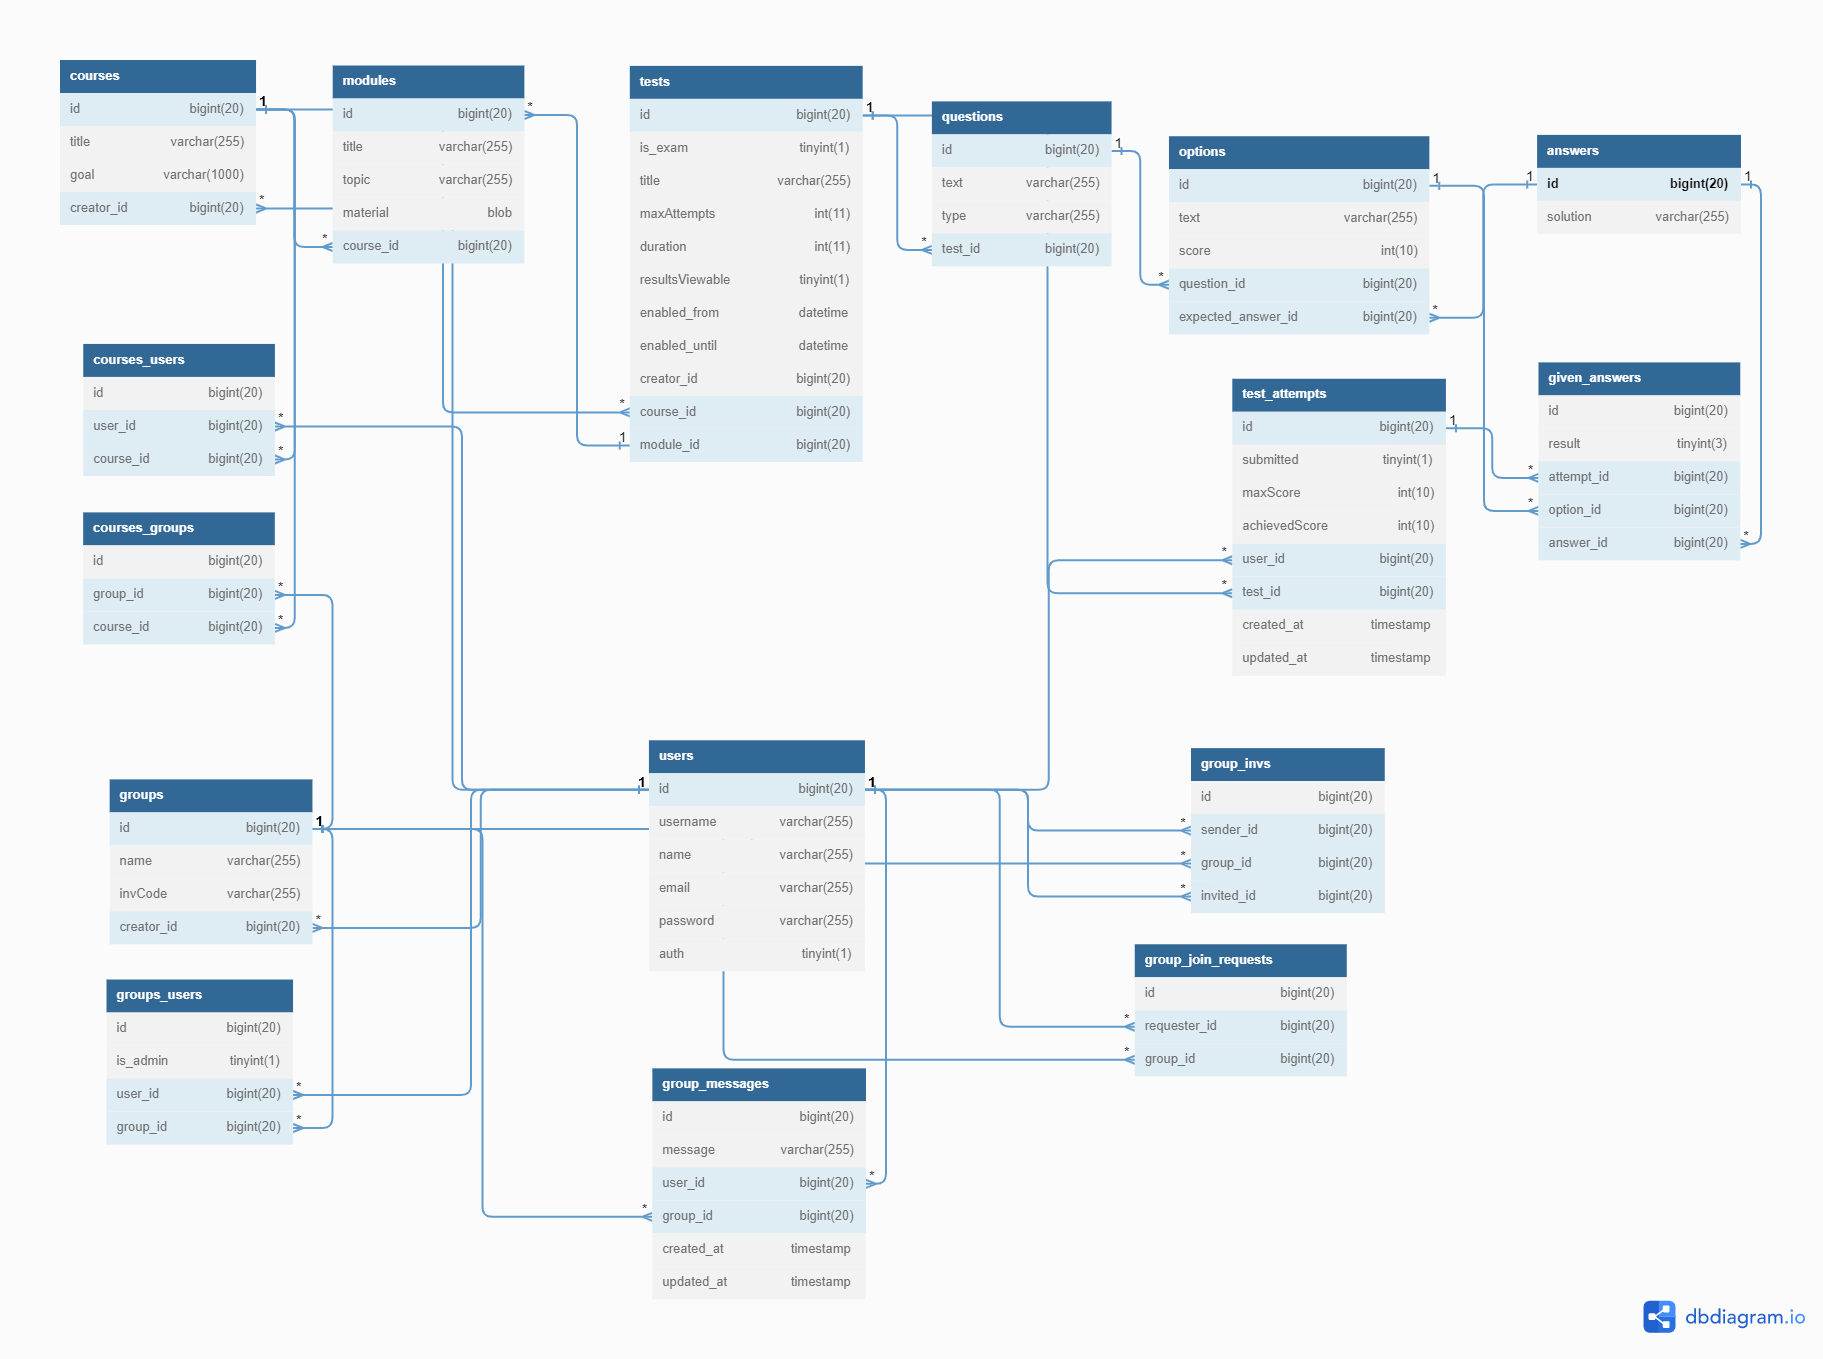
\includegraphics[width=15cm]{Vizsgaztato.png}
		        \caption{Az adatbázis felépítése}
                \label{fig-db-teljes}
	    \end{figure}
            \Az{\ref{fig-db-teljes}} képen látható a teljes adatbázis felépítése. A következő fejezetekben részletezni fogom a táblák közti kapcsolatokat úgy, hogy felosztom két nagyobb szekcióra a projektet.
            \section{A kurzusok felépítése}
                A projekt egyik fő logikai egységét képezik a kurzusok, amelyek azzal a céllal jöttek létre, hogy legyen egy olyan gyűjtő egységünk, amely magába foglalja az egyes órákhoz tartozó tananyagokat (modulok), gyakorló feladatokat (kvízek) és vizsga feladatsorokat.
                \begin{figure}[ht!]
    		        \centering
    		        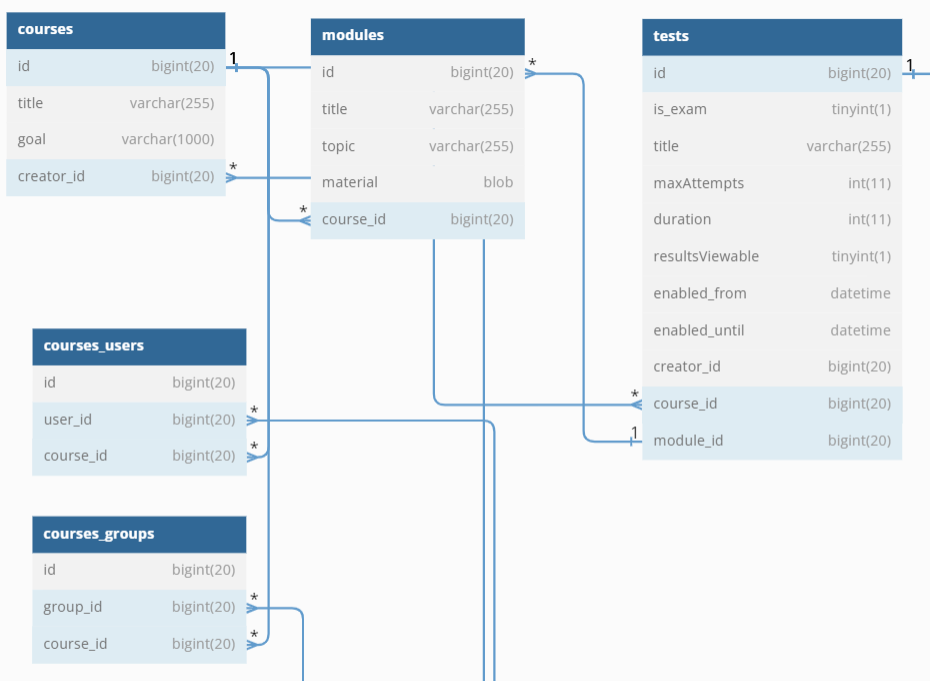
\includegraphics[width=15cm]{Kurzusok_db_1.png}
    		        \label{fig-db-kurzusok-1}
              
    		        \centering
    		        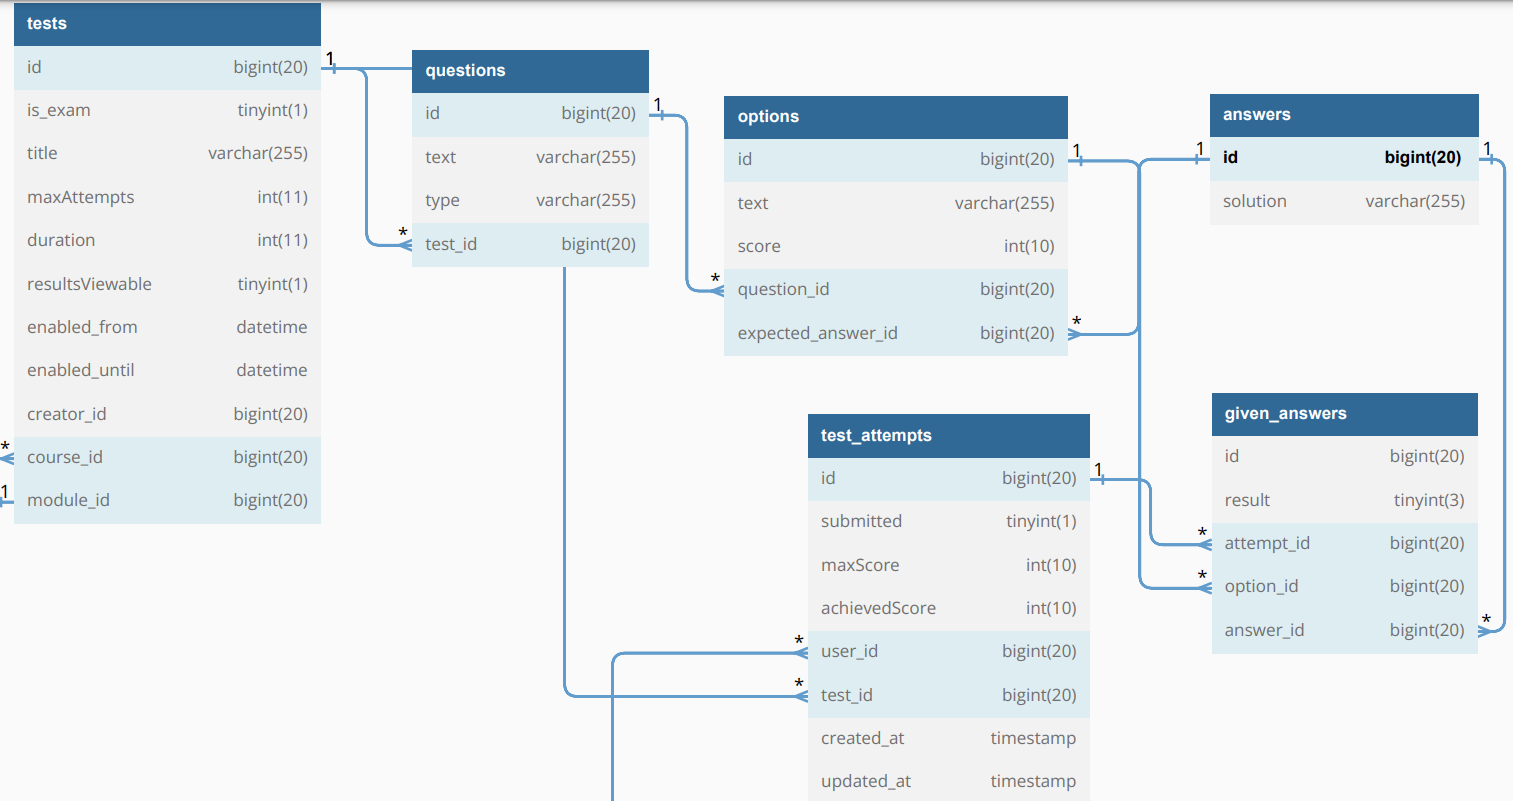
\includegraphics[width=15cm]{Kurzusok_db_2.png}
    		        \label{fig-db-kurzusok-2}
                        \caption{A kurzusokkal kapcsolatos táblák az adatbázisból}
    	    \end{figure}
                \subsection{Kurzus}
                    Minden kurzus rendelkezik egy megnevezéssel, illetve a képzés céljának leírásával. Itt eltároljuk a kurzust létrehozó felhasználó azonosítóját, hiszen csak neki fogunk biztosítani lehetőséget a módosításhoz, a résztvevők kezeléséhez és a törléshez.

                    A kurzusokhoz hozzárendelhetünk embereket -- ez a kapcsolat a ,,\emph{courses\_users}'' táblában fog eltárolódni, ami a \emph{több-a-többhöz} kapcsolathoz létrehozott kapcsolótábla--, illetve csoportokat -- ez pedig a ,,\emph{courses\_groups}''-ban fog rögzítésre kerülni.
                \subsection{Modul}
                    Modulokat tudunk létrehozni a kurzusainkhoz, amik tartalmazzák az egyes órák tananyagait. Az elkészítés során meg kell adni az óra címét, a témakör megnevezését illetve a tananyagot. Itt biztosítjuk az \emph{egy-a-többhöz} kapcsolatot a ,,\emph{modules}'' tábla ,,\emph{course\_id}'' mezőjében.
                \subsection{Teszt} \label{Test-structure}
                    A kétféle teszttípus miatt két idegen kulcsot használunk ebben a táblában: 
                    \begin{itemize}
                        \item Kvízhez: rögzítjük, hogy a teszt melyik modulhoz készült (ez lehet null is, ilyenkor csak szimplán, esetlegesen egy vizsga feladat gyakorlására készülhetett) a ,,\emph{test.module\_id}'' mezőjében.
                        \item Vizsga feladatsorhoz: rögzítjük, hogy melyik kurzushoz készült a ,,\emph{test.course\_id}'' mezőjében.
                    \end{itemize} 
                    Azt, hogy éppen milyen az adott teszt típusa, az ,,\emph{is\_exam}'' boolean mező értékével adhatjuk meg.
                    
                    Ha vizsga feladatsort hozunk létre, megadhatjuk, hogy a kurzushoz rendelt felhasználók és a csoportok tagjai mettől-meddig érhetik el a teszt kitöltését (év, hónap, nap, óra, perc-re pontosan) az ,,\emph{enabled\_from}'' és ,,\emph{enabled\_until}'' mezők segítségével.

                    További, kötelezően megadandó teszt attribútumok: megnevezés (\emph{title}), láthatóak-e a megoldások (\emph{resultsViewable}), kitöltéshez rendelkezésre álló idő percben (\emph{duration}). 

                    Minden teszthez tartozik legalább 1 kérdés (\emph{question}), aminek van:
                    \begin{itemize}
                        \item Szövege
                        \item Típusa (TrueFalse, OneChoice, MultipleChoice, Sequence)
                        \item Több válaszlehetősége (\emph{option}), amiknek attribútumai:
                        \begin{itemize}
                            \item ,,question\_id''-vel eltárolom, hogy melyik kérdéshez tartozik az opció,
                            \item Szöveg (\emph{text}),
                            \item Hány pontot ér (0 vagy 1, \emph{score}),
                            \item Melyik kérdéshez tartozik (\emph{question\_id})
                            \item Elvárt válasz azonosítója (\emph{expected\_ans\_id}). Ezt egy külön táblában, az ,,\emph{answers}''-ben tároltuk el, hiszen így elkerülhető a válaszok nagy mértékű redundanciája
                        \end{itemize}
                    \end{itemize}

                \subsection{Vizsga feladatsor kitöltése}
                    Egy próbálkozás indításánál létrehozunk egy új rekordot a ,,\emph{test\_attempts}'' táblában, ahol eltároljuk, hogy \emph{ki}, \emph{melyik teszthez}, \emph{mikor} kezdte meg a kitöltést. A feladatlap kitöltésének végeztével kiszámoljuk a maximálisan elérhető illetve az elért pontszámokat, amiket szintén eltárolunk. 

                    Az eredmények későbbi ellenőrzéséhez a feladatlapon rögzített válaszokat elmentjük a 
                    ,,\emph{given\_answers}'' táblában, ahol megadjuk, hogy melyik próbálkozáshoz adtuk le az egyes válaszainkat, mi az a válaszlehetőség, amihez tartozik a válaszunk, illetve a diák által adott érték helyes volt-e az elvártakhoz képest, vagy sem.
                    
            \section{A csoportok felépítése}
            \begin{figure}[ht!]
    		        \centering
    		        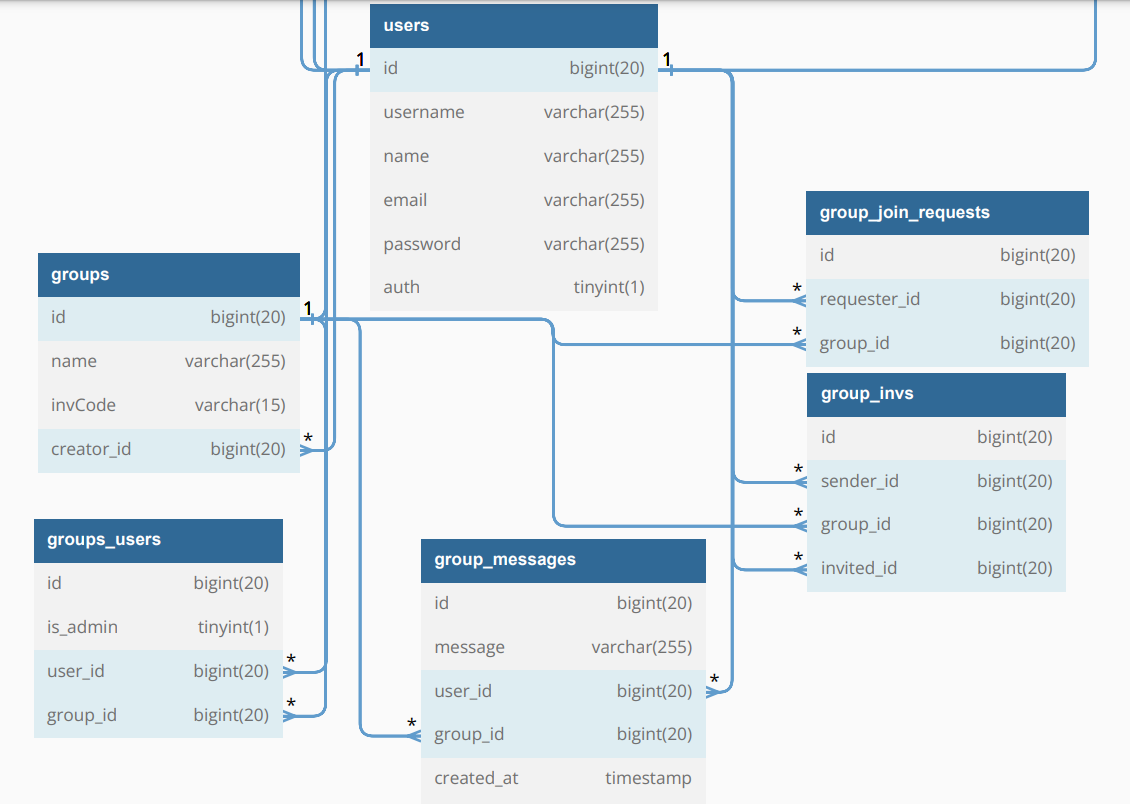
\includegraphics[width=15cm]{Vizsgaztato_csoportok.png}
    		        \label{fig-db-csoportok}
                        \caption{A csoportokkal kapcsolatos táblák az adatbázisból}
    	    \end{figure}
                A másik fő egységet képezik a csoportok, amik segítségével egy valódi közösséget tudunk teremteni mind a diákok, mind a tanárok körében úgy, hogy egy csevegő felület segítségével kommunikálhatnak egymással a csoport tagjai. Ezek mellett arra is nagyszerű megoldás, hogy egyszerűsítsük a tanulóknak a kurzusokhoz való hozzárendelés folyamatát, hiszen ennek segítségével egyszerre több tanulónak is elérhetővé tehetjük a tananyagainkat.
                

                A csoportról csupán néhány információt tárolunk el a \emph{groups} táblában:
                \begin{itemize}
                    \item Mi a neve? (\emph{name})
                    \item Meghívó kód (automatikusan generált, \emph{invCode}) 
                    \item Ki hozta létre? (\emph{creator\_id})
                \end{itemize}
                
                Két csatlakozási lehetőséget biztosítottam a felhasználók számára:
                \begin{itemize}
                    \item A felhasználó egy adott csoport egyedi meghívó kódját elküldve rögzíti jelentkezési kérelmét a ,,\emph{group\_join\_requests}'' táblában, amit majd később a csoport tulajdonosa vagy elfogad, vagy elutasít.
                    \item A csoportot létrehozó felhasználó a kereső segítségével meginvitálja az adott csoportba a kikeresett felhasználó(ka)t. Ilyenkor a kérelem/kérelmek a ,,\emph{group\_invs}'' táblában kerül eltárolásra, ahol megtudjuk, hogy ki hívott meg (\emph{sender\_id}) kit (\emph{invited\_id}) és milyen csoportba (\emph{group\_id}).
                \end{itemize}

                Amint a csoport tagjaivá válunk, elérhetővé válik számunkra egy ,,Üzenetek'' felület, aminek adatait a ,,group\_messages'' táblában tároljuk.

        \chapter{A projekt megvalósítása}
        	Ebben a fejezetben a projektben alkalmazott technológiát mutatom be úgy, hogy a Laravel alap működését magyarázom el példák segítségével, kitérve arra, hogy mit, miért és hogyan implementáltam.
 
            \section{A Laravel alap működése}\label{Laravel-mukodes}
                \subsection{Migration}
                    A Laravel Migration-je\cite{Laravel-Migrations} egy egységes sémát biztosít az adatbázisunk tábláinak a felépítésére, amelyet megoszthatunk a projekten dolgozó többi fejlesztővel. Ez azért kifejezetten hasznos, mert a manuális tábla-módosítás helyett csupán csak a módosított migration-t kell futtatni, így amellett, hogy energiát és időt spórolunk meg, sokkal kisebb az esetleges emberi pontatlanságokból adódó hibák száma.

                    Egy migration-t legegyszerűbben a \emph{php artisan} segítségével generálhatunk le. A létrehozott fájlunkon belül található ,,up'' metódusban meghatározzuk a táblánk nevét, illetve annak egyes attribútumait úgy, hogy a kívánt típusnak megfelelő metódus hívást elvégezzük, majd paraméterként átadjuk a mezőnek szánt nevet illetve egyéb megkötéseket (például hossz).
                    \lstinputlisting[caption=Példa egy migration-re a projektből.]{migration.php}
                    Az egyszerűbb kapcsolatkezelés végett a Laravel egyik alap konvenciója, hogy a külső kulcsokat az összetartozó táblának egyes számú nevével és az ,,\_id'' felirattal lássuk el, erre a példa migration-ből:

                    A ,,\emph{group\_message}'' tábla kapcsolatban van a ,,\emph{groups}'' és ,,\emph{users}'' táblával, ezért az idegen kulcsok ,,\emph{group\_id}'' és ,,\emph{user\_id}'', így a modelljeinken belüli kapcsolatok meghatározásánál nincsen szükség további pontosítások megadására. 

                    A projektben több olyan eset is volt, amikor nem követtem ezt a konvenciót, nemes egyszerűséggel az olvashatóság végett. Ez semmi negatívummal nem jár azon kívül, hogy a kapcsolatok meghatározásánál meg kell még adnunk néhány külső és helyi kulcsot.

                    Az elkészített migration-jeinket szintén a php artisan-nak a \emph{migrate} parancsával tudjuk futtatni, s így létrejönnek a migrációs állományokban meghatározott táblák.
                    
                \subsection{Model}
                    A keretrendszerünk biztosít számunkra egy Eloquent ORM-et\cite{Laravel-Models}, ami segít abban, hogy általunk definiált osztályokon tudjunk elvégezni különböző metódus hívásokkal adatbázis-műveletek sokaságát a kontrollereinken belül.

                    Alapértelmezetten a modellünk a tábla-összeköttetést az osztály nevének megfelelően úgynevezett ,,snake\_case'' konvenció szerint fogja összekötni, ami annyit teszt, hogy egy \emph{PéldaOsztály} modellt egy \emph{példa\_osztály} nevű táblával kötne össze. A rekordjaink azonosítóját (primary key) is \emph{id}-ként fogja keresni, hacsak nem határozzuk meg explicit módon, hogy eltérünk a megszokottaktól.

                    A ,,\emph{\$fillable}'' protected mezőben kell felsorolnunk azokat a mezőket, amelyeket kulcsokként kívánunk alkalmazni a \emph{create} és \emph{update} metódusoknak paraméterként átadott asszociatív tömbön belül.

                    A modellen belül szükségeltetik megadni azokat a kapcsolatokat is, amelyek az adott modellünkhöz tartoznak. Legyen Egy-az-Egyhez, Több-az-Egyhez vagy Több-a-Többhöz kapcsolat, könnyedén definiálhatjuk a megfelelő metódusok hívásának (hasOne - belongsTo, hasMany - belongsTo, belongsToMany) a megfelelő paraméterezésével, ahol az elnevezési konvenciók követésével csak a kapcsolódó modell nevére van szükségünk, egyébként pedig általában egy esetleges kapcsoló tábla, külső- és helyi kulcs megadására lesz szükségünk.
                    
                \subsection{N+1 Query Problem}
                   Az összetettebb kapcsolatok megjelenítését eleinte a nézeteken használt ciklusok magjában oldottam meg úgy, hogy a kívánt kapcsolatot lekérdeztem minden vizsgált elemen, ezzel egy úgynevezett ,,Lazy Loading''-ot megvalósítva, ami performancia hibákhoz vezethet sok adat esetén. Később a Laravel Debugbar\footnote{Laravel Debugbar: \url{https://github.com/barryvdh/laravel-debugbar}} segítségével kiderült, hogy sokkal több lekérdezést hajtok végre az oldal betöltése során, mint amennyire igazából szükség lenne. 

                    A probléma magyarázata: 
                    \begin{itemize}
                        \item Végrehajtok \textbf{1} lekérdezést az adatok kinyerésére
                        \item Az \textbf{N} db visszaadott rekodnál szintén kiadok 1-1 lekérdezést a ciklusok lefutása során
                    \end{itemize}
                    Ekkor az a probléma, hogy egy összetettebb lekérdezés (például INNER JOIN) helyett N + 1 kisebb query-t küldünk az adatbázisunknak, ami a visszakapott adatok mennyiségével arányos módon ronthatja az oldalunk teljesítményét.
                    
                    A probléma elhárításához a Laravel biztosít egy kapcsolatot, ami az \emph{Eager Loading}. Ennek segítségével a modellek kinyerésekor megszabhatjuk, hogy milyen további, már meghatározott kapcsolatot kívánunk vele összekötni -- ilyenkor a háttérben egy egyszerű INNER JOIN-t használ --, így egyetlen lekérdezéssel kinyerhetünk minden szükséges adatot a megjelenítéshez, amit módosítás nélkül meg tudunk jeleníteni az oldalon. 

                    Ha egy lekérdezést akarunk elvégezni a táblánkon, akkor a \emph{Model} osztály \emph{with} statikus függvényét kell meghívnunk, ahol paraméterben átadjuk a modellünk kapcsolatát/kapcsolatait. Itt lehetőségünk van arra, hogy  felsoroljuk a szükséges relációkat, valamint a ,,Nested Eager Loading''-gal az is, hogy mélyebb kapcsolatokat is egyetlen paraméterrel lekérdezzünk.

                    Tehát ha ki akarom nyerni a legutolsó csoportüzenetet a küldő adataival együtt, akkor \az{\ref{EagerLoadingExample}}.~kódban leírtakat kell tennem:
                    \lstinputlisting[caption=Eager Loading-ra példa., label=EagerLoadingExample]{EagerLoadingexample.php}

                    Ha egy lekérdezést akarunk elvégezni egy \emph{meglévő modellen}, akkor a \emph{Model} osztály \emph{load} példányszintű függvényét hívjuk, ahol a paraméterezés ugyanúgy működik, mint a fentebb említett metódusnál.

                    \Az{\ref{LazyEagerLoadingExample}}.~kódban egy, a paraméterből érkező kurzusnak kérdezem le a hozzárendelt felhasználóit, csoportjait és kvízeit:
                    \lstinputlisting[caption=Lazy Eager Loading példa., label=LazyEagerLoadingExample]{LazyEagerLoadingexample.php}
                    
                \subsection{Controller}
                    A \emph{web.php} fájlokban előre definiált útvonalaknak megfelelően végezhetünk anonim metódushívásokat, aminek a törzsében elvégezhetjük az útvonalnak meghatározott feladatokat, viszont ez túlságosan átláthatatlan kódhoz vezet. A jobban struktúrált kód végett hasznos, ha a kérelmeket kezelő logikát Controller-ekbe\cite{Laravel-Controllers} helyezzük el és ezeknek az egyes metódusait hívjuk meg a route-ok kezelésekor.

                    Jellemző, hogy a legtöbb Migration-höz egyszerre generálunk Model-t és Controller-t is, így az egyes objektumokon végzendő logika mindig jól meghatározott és elkülönült helyen található úgy, hogy a rendszer elnevezésekkel kapcsolatos konvenciókjait is betartja.

                    A Controller-ben tipikusan egy (vagy több, a vizsgált objektumunkhoz tartozó) Model osztállyal dolgozunk. Ennek biztosítjuk az alapvető CRUD műveleteket:
                    \begin{itemize}
                        \item Create - 2 metódus:
                            \begin{itemize}
                                \item create(): a létrehozáshoz szükséges űrlapot tartalmazó nézetet adja vissza.
                                \item store(Request \$request): a create űrlapjáról érkező adatokat kiolvassuk \emph{\$request} változóból és azok alapján létrehozunk egy objektumot.
                            \end{itemize}
                        \item Read - 2 metódus:
                            \begin{itemize}
                                \item index(): lekérdezzük a kontrollerben kezelt modell minden, az adatbázisban található példányát, majd ezeket átadjuk megjelenítésre az index által visszaadott nézeten.
                                \item show(Model \$model): a paraméterből érkező példányt küldjük át megjelenítésre a nézetre.
                            \end{itemize}
                        \item Update - 2 metódus:
                             \begin{itemize}
                                \item edit(Model \$model):  a paraméterből érkező példányt adjuk át a nézeten elhelyezett űrlapra, ami általában megegyezik, vagy legalább is nagyon hasonló a \emph{create} oldalhoz, viszont az átadott változó mezőit betöltjük az \emph{input mezőink} értékeibe.
                                \item update(Request \$request, Model \$model): az edit űrlapjáról érkező adatokat kiolvassuk a \emph{\$request} változóból és azok alapján a második paraméter mezőit frissítjük és mentjük.
                            \end{itemize}
                        \item Delete - 1 metódus:
                        \begin{itemize}
                         		\item destroy(Model \$model): a paraméterből érkező modellt kitöröljük az adatbázis rekordjai közül.
                        \end{itemize}
                    \end{itemize}

                    Egy bevált módszer az is, hogy a Controller helyett egy Resource-t generáltatunk a \emph{php artisan}-nal. Ez biztosítja a fentebb említett 7 metódust, importálja és paraméterezi a használni kívánt Model-lel a metódusainkat és kommentjeinket. A generált Resource-unkat lehetőségünk van behivatkozni a \emph{route.php}-n belül, ahol alapból kapni fog minden egyes route egy egyedi nevet, jellemzően a metódus nevének megfelelően.

                    A route-okhoz biztosított egy lehetőség, amivel elkerülhetjük a hosszas útvonalak leírását azzal, hogy a hivatkozás meghatározásánál egy \emph{name} függvény paraméterében megadjuk, hogy milyen egyedi névvel szeretnénk rá hivatkozni a későbbiekben.
                    
                \subsection{Refaktorálási kísérletek}
                    A fejlesztés során beleestem egy olyan hibába, amit a hozzám hasonló, kevés szakmai gyakorlattal rendelkező programozók is gyakran elkövetnek: túlságosan hosszú és átláthatatlan kódot írtam úgy, hogy nem használtam ki a keretrendszer által biztosított lehetőségeket.

                    Az őszi félév elején elkezdtem dolgozni a projekten, viszont inkább az óráimra készültem, ezért nem tudtam olyan sűrűn foglalkozni vele, ahogy kellett volna. Amikor kisebb-nagyobb kihagyások után visszatértem, előfordult, hogy elszörnyülködtem, hogy a 2-3 hete írt kódomat egyszerűen nem tudom értelmezni. Nem értettem, hogy mit csinál, milyen logikát követ, mit hivatott elintézni.

                    Hosszú, egymásba ágyazott ciklusokkal teli kontrollerek, nem megfelelő elhelyezése a különböző logikáknak, nem teljesen átgondolt elvárások a programmal szemben. Szerencsére rátaláltam egy Laravel Daily nevű csatornára, ahol egy közel 20 részes lejátszási lista volt elérhető Junior Code Review\cite{LaravelDaily - CodeReview} különböző aspektusokra fókuszálva.

                    Ennek a tanulmányozása előtt már megkezdtem az Eager Loading használatát, amivel már jó pár foreach-től megszabadultam, viszont még mindig elfogadhatatlan volt a kód minősége, így továbbra is szükséges volt a kontrollerek újradolgozása.

                    \subsubsection{Events \& Listeners}
                    A videók többségének megtekintésével illetve a témakör után olvasgatva úgy véltem, hogy két opcióm van olyan problémák megoldására, amik bizonyos események lefutásához kapcsolódnak: Observer vagy Event-Listeners.
                    
                    Megismerkedtem a Laravel \emph{Observerével}, viszont hosszú távon nem tűnt túlságosan átláthatónak használata ahhoz, hogy fenntartható kódot írjak. Tegyük fel, hogy egy hónapokkal későbbi debugolás vagy refaktorálás során valószínűleg meggyűlne a bajunk, ha egy tőlünk valamennyire ,,elrejtett'' logikát kellene észrevennünk, hogy az valami módosítást hajt végre a programunk valamely más részén. 
                    
                    Ezért is döntöttem úgy, hogy inkább az \emph{Event-Listener}\cite{Laravel-Events, Laravel-EventsExample} megvalósítást használom, aminek a működése felettéb hasonlít az előbb említett Observer-éhez azzal a különbséggel, hogy itt nekem kell explicit módon egy eseményt kiváltani egy általam meghatározott helyen, viszont ezeknek hívását ugyanúgy lekövetik a Listener osztályaink.
                    
                    Ezt például a csoportok létrehozásánál használtam, ahol is:
                    \begin{itemize}
                    	\item A GroupController \emph{store} metódusában kiváltok egy ,,\emph{GroupCreated}'' eseményt, aminek paraméterül átadom a létrehozott csoport példányt.
                    	\item Az ,,\emph{EventServiceProvider}.php''-ben ehhez az eseményhez hozzárendeltem egy \emph{listener} osztályt, aminek a neve ,,\emph{AddFirstUserToGroup}''.
                    	\item Az ,,\emph{AddFirstUserToGroup.php}''-on belül található \emph{handle} metódus paraméterében található esemény kiváltása után kiolvasom az eseményből érkező adatokat (csoport azonosító), majd az alapján elvégzem a létrehozó felhasználó hozzáadását a csoporthoz. 
                    \end{itemize}
                    
                    \subsubsection{Services és Actions}
                    Olyan hosszadalmas programkódot, ami nem feltétlen kellett az egyes controllerekbe -- mert vagy nem az adott controller modelljén hajtott végre valamilyen műveletet, vagy inkább segédszámítások és átalakítások elvégzéséhez kellett --, kiszerveztem vagy egy Service, vagy egy Action osztályba. Ilyen volt például a tesztek összeállítását végző eljárás, ami olyan formában adta vissza a modellt, amely átadható a Livewire komponenseknek, vagy egy teszt kitöltését rögzítő művelet. Így egy több tíz soros logika helyett elintézhető egyetlen sorral a művelet, növelve ezzel is a kontrollerem függvényének átláthatóságát, valamint az egyes komponensek újrahasználhatóságát is megvalósítottam ezzel.

                    \subsubsection{Requests}
                    A form-okból érkező adatok feldolgozása illetve a kontrollerben lévő validációs folyamatok szintén megnövelték a kontrollerjeim méretét -- mint utólag kiderült, teljesen feleslegesen. 
                    
                    A dokumentációt olvasva megtudtam, hogy egyszerűbben meghatározhatom az egyes validációs lépéseket és a hozzájuk tartozó hibaüzeneteket is egy saját Request osztályban. Ezért a legtöbb formokat feldolgozó metódusok paraméterében az alap ,,\emph{Request}'' osztály helyett az általam létrehozott egyedi kérésvalidációs állományt használtam.

                    Itt meghatároztam különböző, az input mezőkhöz tartozó korlátozásokat (required, minimum-, maximum hossz, típus) és azok hibaüzeneteit. Viszont most szükség volt arra is, hogy ezeket megjelenítsem a formjaim oldalán is, hiszen másként nem tudom informálni a felhasználót az általa elkövetett hibákról. 
                    
                    Ezt a legtöbb oldalon úgy végeztem el, hogy a form tetején kiiratom az összes, \emph{\$errors->all()} által visszaadott hibaüzenetet, ha az \emph{\$errors->any()} igazzal tér vissza, tehát van lekezelendő validációs hiba.

                    Másik lehetőség a Laraveles \emph{@error} direktíva, amiről \az{\ref{LivewireRealTimeValidation}}.~bekezdésben fogok még írni.
                    
                    A modelljeink létrehozását és frissítését végző programkódjaink rövidítésére van egy további alternatívánk is egy saját Request létrehozásával. Ilyenkor a paraméter ,,\emph{\$request}'' változójával egyetlen sorban elvégezhetjük az utasításokat, mégpedig úgy, hogy a ,,\emph{\$request->validated()}'' által visszaadott asszociatív tömböt átadjuk paraméterként a frissítést vagy létrehozást végző függvényünknek. 
                    
                    Például: \emph{\$course->update(\$request->validated());}
                    
                \subsection{View és Blade fájlok}
                    Az MVC által használt nézetekhez a Laravel biztosít úgynevezett Blade sablonokat. Ezek az oldalak a legtöbb esetben a Controller-ek által kerülnek megjelenítésre a felhasználóinknak, viszont nem idegen dolog az sem, amikor a route-ok lekezelésekor adunk vissza egy-egy nézetet.

                    A nézeteinket a ,,\emph{resources/views}'' könyvtárban találhatjuk meg. Észrevehető, hogy ezen belül is van egy ,,\emph{layouts}'' directory, amin belül kerülnek elhelyezésre azok az alap sablon fájlok, amik tartalmazzák a teljes projektre tartozó hivatkozásokat (például külső CSS és JS fájlok), növelve ezzel a komponenseink újrahasználhatóságát és csökkentve a kódismétlést.

                    Mivel ezek a blade fájlok is PHP kiterjesztésűek, ezért tartalmazhatnak a megszokott módon PHP-n kívül HTML, CSS és JavaScript kódokat is.

                    A kontrollerből érkező adat(oka)t egy sajátos szintaxissal, az ,,echo statement''-tel tudjuk megjeleníteni úgy, hogy ,,\{\{~~\}\}'' zárójelpárok között megadjuk a megjelenítendő változó nevét, ami a következő módon nézne ki cím kiiratásnál:
                     \lstinputlisting[caption=Példa az echo statement-re]{EchoStatement.php}

                    A blade fájlok további előnye, hogy lehetővé teszik a fejlesztők számára, hogy egyszerűbb módon alkalmazzanak vezérlési szerkezeteket (például ciklusokat vagy elágazásokat) a beérkező adatok dinamikus megjelenítéséhez. Ezeket az utasításokat előre meghatározott direktívák\cite{Laravel-BladeDirectives} alkalmazásával hajthatjuk végre. Rendkívül pozitív a használatuk során, hogy a PHP-ban már jól megszokott szintaxisokat kell itt is használnunk, valamint a kód olvashatóságát is növelik, hiszen nem kell külön bajlódnunk a PHP tag-ek alkalmazásával a különböző hívások elvégzéséhez.
                    \lstinputlisting[caption=Példa egy if-es blade direktívára]{BladeIfDirectiveExample.php}

                    Egy jól bevált szokás, hogy kialakítunk egy ,,szülő-gyermek'' struktúrát\cite{Laravel-BladeLayoutInheritance} az oldalak között úgy, hogy egy alap sablon (egyik layout-beli view) különböző részeibe hivatkozunk be más, a kontrollerjeink által visszaadott nézetnek a különböző, alap sablonnak megfelelő szekcióit.

                    Ezt úgy tudjuk elvégezni, hogy definiálunk egy ,,szülő'' fájlt, amely tartalmazza a projektünk főbb hivatkozásait és tulajdonságait (például háttérszín, behúzások, külső fájlok). Itt megszabunk bizonyos részeket, amiket a ,,gyermek'' nézetektől várunk el, hogy átadjanak. Ilyen mondjuk az oldalaink címei vagy a megjelenítendő tartalmuk.

                    Tegyük fel, hogy létezik egy alap sablon nézet, amely a ,,\emph{resources/views/layouts}''-ban található \emph{app\_example.blade.php} fájl, amelyben elvárjuk a ,,\emph{@yield('...')}'' direktívával, hogy adott kulccsal beszúrásra kerüljenek a gyermek nézetnek az elemei.
                    \lstinputlisting[caption=app\_example.blade.php példa kódja]{app\_example.blade.php}

                    Ehhez írnunk kell egy ,,gyermek'' oldalt, amely szolgáltatni fogja a ,,szülő'' nézet hiányos részeit a ,,\emph{@section('...')}'' direktívával miután megmondtuk, hogy melyik oldalt is terjeszti ki (\emph{@extends('...')}'').
                    \lstinputlisting[caption=app\_example.blade.php példa kódja]{view\_example.blade.php}
                    
            \section{Autentikáció}
                \subsection{Laravel/UI}
                Mivel egy picit korábbi projektem folytatása ez a webes vizsgáztató rendszer, ennélfogva egy akkoriban általam jól megszokott csomagot használtam a felhasználói azonosításra, ami a \emph{laravel/ui} package. A telepítésének és használatának a részletes leírása az online dokumentációban\cite{Laravel-7Auth} volt elérhető, tehát nem jelentett nagyobb gondot a használata. Egyetlen problémája az volt, hogy Bootstrap-et használt a Tailwind helyett, viszont az osztályok átírása gyorsan megoldható volt, így nem kellett akkoriban alternatívák után kutatgatni. 

                A szakdolgozat fejlesztése közben láttam, hogy már az új, Laravel 10.x-es online dokumentáció\cite{Laravel-10Auth} a \emph{Laravel Breeze} csomagot ajánlja. Ez is a laravel/ui-hoz hasonlóan blade fájlokat használ és szinte ugyanolyan eljárású kontrollereket. Mivel a UI és Breeze ugyanolyan azonosítást használ és a végrehajtott eljárásaik is nagyon hasonlóak, maradtam a UI-nál.

                Nagy előnye, hogy kapunk jó néhány előre megírt komponenst:
                \begin{itemize}
                    \item Controller-ek: Auth könyvtárban 6 kontroller, pl. Login-, RegisterController.php
                    \item View-ok: szintén 6 nézet az auth directory-ban, pl. login, register, verify.blade.php
                \end{itemize}
                Ezek anélkül is teljesen működnek, hogy akármit is módosítani kellene rajtuk, viszont igény szerint bővíthetőek is. Sajnos ilyenkor mind a User modellt, mind a ,,users'' migration-t is módosítanunk kell a változtatások helyes lekövetéséhez, valamint a csomaghoz tartozó PHP fájlokban is módosításokat kell végrehajtanunk.

                Szóba jöhetett volna még a Fortify, esetleg a Jetstream\cite{Laravel-AuthComparison} csomag is, viszont nem igazán tudtam volna kihasználni az általuk biztosított lehetőségeket, illetve mindenképpen maradni szerettem volna a blade fájlok használatánál a Livewire komponensek helyett.
                
                \subsection{Middleware}
                A Laravel Middleware-je egy köztes átjáróként (Gate)-ként szolgál a HTTP kérések és az őket feldolgozó route-ok között. Különböző feltételeket szabhatunk az applikációnk felé érkező kéréseknek annak érdekében, hogy azokat egyáltalán feldolgozzuk és eljuttassuk a web.php-nk felé.

                Az előre definiáltak közül az egyik ilyen middleware, amit használtam az ,,\emph{auth}'', amely a felhasználói azonosításért felel. Ez biztosítja, hogy az oldalaimat csak akkor érhessék el a userek, ha sikeresen bejelentkeztek, egyébként visszadobja őket a login page-re. A másik ilyen a ,,\emph{verified}'', amely megkötelezi az összes usert, hogy az email címükre érkező levélben található hivatkozással erősítsék meg a regisztrációjukat.
                
                Az egyes állapotok megkülönböztetéséhez a Laravel biztosít nekünk  például egy \emph{@guest} direktívát, ami igazából egy elágazásként is szolgálhat. Ennek a törzsébe akkor lépünk be, ha még nem történt felhasználói bejelentkezés, az ehhez írható @else ágba pedig akkor, ha sikeres volt az azonosítás. Ilyen módszerrel vannak meghatározva a navigációs sávon belül elérhető oldalhivatkozások is.

                Az alkalmazásunk bejelentkezett felhasználóinak elérésére kapunk egy helper function-t is, ami az \emph{auth()}. Ezzel lekérdezhetjük a szerver oldalon eltárolt munkamenetből a böngészőnk sütijei segítségével a bejelentkezett User Model-jét (\emph{auth()->user()}), vagy csak egyszerűen annak azonosítóját (\emph{auth()->id()}). Ez azért ajánlatos a Facade-ból beimportálható Auth osztállyal szemben, mert így biztos nem fordul elő, hogy elfelejtünk egy hivatkozást, valamint a blade-jeinken belül is szabadon használható.

                További lehetőségünk van arra is, hogy a route-jainkat csoportosítsuk a rájuk vonatkozó middleware-eknek megfelelően, ahol akár felsorolásszerűen is megadhatóak a szabályrendszerek, elkerülve ezzel a további kódismétlést.
                \lstinputlisting[caption=web.php-ban található Middleware hívás, label=routeCode]{web.php}
                \Az{\ref{routeCode}}.~kódban kötelezzük a felhasználókat a bejelentkezésre, illetve a bejelentkezett usereinket arra, hogy megerősítsék az email címűket az oldal útvonalainak teljes eléréséhez.
                
                \subsection{Szabályzatok (Policies)}
                A felhasználók által végrehajtható műveleteknek a szabályozására a keretrendszerünk biztosít egy eszközt a fejlesztőknek, amit Policy-nek\cite{Laravel-AuthPolicies} neveznek. 
                
                Ezek szintén generálhatóak a php artisannal, amely minden egyes CRUD művelethez létrehoz 1-1 ellenőrző függvényt, amelynek beérkező \emph{\$user} paraméterével eldönthetjük, hogy a megadott (bejelentkezett) felhasználóra milyen szabályrendszert szeretnénk felállítani az adott művelet elvégzéséhez. Az ilyen fájlokat az ,,\emph{app/Policies}'' könyvtárban találhatjuk meg.
                
                Egy policy függvénynek visszatérésének két kimenetele lehet. Vagy egy engedélyező (\emph{Response::allow()}) választ kapunk a policy-tól, vagy elutasítót, amelyben egy megadott üzenetet is meghatározhatunk (\emph{Response::deny('Elutasító üzenet')}.

                Az alábbi példával egy try-catch segítségével próbálkozni fogunk egy teszt törlésével. Ha nem megengedett a megadott művelet, visszatereljük a felhasználót egy index oldalra egy SweetAlert-es felugró ablakkal, ahol informáljuk, hogy nem engedélyezett műveletet próbált meg végrehajtani. 

                Amennyiben viszont egy felhatalmazott személy próbálja elvégezni a törlést, a tesztet eltávolítjuk és visszaküldjük az előző oldalra egy megerősítő üzenettel.

				\lstinputlisting[caption=TestPolicy delete metódusa]{DeleteTestpolicy_example.php}
                \lstinputlisting[caption=A TestPolicy függvényét felhasználó TestController destroy metódusa]{DeleteTest_example.php}

                A blade fájljainkon belül is található ezeknek használatához egy direktíva. A ,,\emph{@can}'' paraméteréül meg kell adnunk egy Policy-ra való hivatkozást, így a visszatérő értékeknek megfelelően felhasználói felületen megjelenő elemek közül el tudjuk dönteni, hogy a jogosultságnak megfelelően megjelenítünk-e például egy szerkesztést vagy törlést biztosító gombot, vagy sem.
                
                Például: \emph{@can('delete', \$course)}, ahol leellenőrzöm, hogy a bejelentkezett felhasználó törölheti-e az adott kurzust.

                Minden olyan művelethez használtam a projekten belül, ahol ez indokolt volt.

                
            \section{Livewire működésének megértése}\label{Livewire}
                Mint korábban említettem, a Livewire egy kifejezetten Laravelhez fejlesztett full-stack keretrendszer, amely lehetővé teszi, hogy saját komponensek készítése után beépített AJAX hívások segítségével dinamikusan tudjak oldalakat kezelni anélkül, hogy bonyolultabb JavaScript kódokat írnék.
                \subsection{Oldalak feldolgozása}
                A Livewire komponensek egy nézetből és egy kontrollerből épülnek fel, amelyek szoros összeköttetésben állnak egymással. A komponensünket be kell hivatkozni egy olyan helyen ahol fel szeretnénk azt használi, méghozzá az alábbi módon: \emph{@livewire('group-chat', ['group'=>\$group])}. A példában meghívtuk a csoportos üzenetküldést biztosító komponenst az ,,\emph{@livewire}'' direktívával. Első paraméterben átadásra kerül a komponensünk neve, majd ezt követi a változók felsorolása, ami jelen esetben az, hogy melyik csoport üzeneteit szeretnénk látni.

                A komponens hívásakor egyszer lefut a ,,\emph{mount()}'' függvény, amely arra szolgál, hogy a komponenseinket alaphelyzetbe állítsuk, illetve a komponens hívásánál beérkező adatokat kimentsük egy-egy publikus változóba.

                Ezután pedig a ,,\emph{render()}'' függvény a szerveroldalon előállítja a megjelenítendő oldalt, majd ezt visszaadjuk a blade sablonfájlunknak. Minden alkalommal, amikor a felhasználó érintkezik az oldallal, egy kérés kerül elküldésre a szerver felé, aminek hatására újra meghívódik a \emph{render} metódus, így biztosítva azt, hogy mindig az aktuális adatokat jelenítjük meg a a felületeinken.

                A Livewire további függvényeket is biztosít, amelyek az oldal egyes életciklusaihoz tartoznak. Ilyen például az ,,\emph{updated()}'' függvény. Ezt általában akkor szoktuk alkalmazni, amikor valós idejű validációt szeretnénk megvalósítani az oldalon. Amikor a felhasználóink a bemeneti mezők értékeit változtatják, először ez a függvény hívódik meg, ahol elvégezzük a szükséges műveleteket, majd annak megfelelően újra rendereljük az oldalt.
                \subsection{Tulajdonságok (Properties)}\cite{Livewire-Properties}
                A komponensek nézetein megjelenítendő bemeneti mezők értékeit összeköthetjük 2 irányú ,,data binding''-gal, ami annyit tesz, hogy ha van egy publikus változónk a Livewire kontrollerünkön belül, akkor azt az oldalon lévő input mezővel összeköthetjük a ,,\emph{wire:model="variable\_name"}'' attribútum segítségével. Ilyenkor minden, az input mező értékén végrehajtott módosítás esetén egy-egy AJAX kérés kerül elküldésre a szerver felé, aminek határása a kontrollerben lévő, összekötött változó értéke leköveti a változásokat az aktuális értékre. Fontos megemlíteni, hogy ez a kapcsolat visszafelé is igaz, hiszen ha a PHP kódunkban a változó kezdőértékét módosítjuk, abban az esetben az oldalon is leköveti az input mezőnk értéke a változást.

                Annak érdekében, hogy ne történjen meg az, hogy minden egyes billentyű leütésre küldünk egy kérést a szerver felé, -- ezzel fölösleges hívásokkal terhelve azt --, lehetőségünk van arra, hogy úgynevezett ,,\emph{debouncing}''-gal lecsökkentsük a kérelmek számát. Ez úgy valósul meg, hogy csak azután kerül elküldésre az AJAX kérés, amiután egy előre meghatározott (alapból 150 ms) ideig a felhasználó nem módosít az input mezőnk értékén. Ennek használata a fentebb említett ,,wire.model'' kiegészítésével történik: ,,\emph{wire:model.debounce.150ms="variable\_name"}''

                Abban az esetben, ha csak akkor szeretnénk adat-összeköttetést végezni, amikor már biztosan befejezte a felhasználó a bemenet módosítását, használjuk a ,,\emph{lazy updating}''-ot, ami az alábbi: ,,\emph{wire:model.lazy="variable"}''. Ebben az esetben csak akkor küldjük el a kérést a szerver felé, amennyiben a bemeneti mezőből kikattintott a user vagy az ENTER billentyű lenyomásra kerül.

                Ha a lehető legkevesebb üzenetküldést szeretnénk kivitelezni, akkor használjuk a ,,\emph{wire:model.defer="variable\_name"}'' módszert. Ebben az esetben csak akkor történik meg az értékek szinkronizálása, amikor egyéb okok miatt egy AJAX hívás kerül elküldésre a Livewire felé. Ezzel el tudjuk végezni, hogy eltároljuk az összes módosítást, majd a legvégén egyetlen nagyobb AJAX hívást küldve a szerver felé validálunk minden adatot és azoknak megfelelően intézkedünk a lefutás további részében.
                
                
                \subsection{Műveletek és Események (Actions \& events)}\cite{Livewire-Actions, Livewire-Events}
                Az input mezők összeköttetésén kívül van egyéb lehetőségünk is Livewire-es hívást intézni. Ezek közül egyik ilyen az ,,action'', ami segítségével könnyedén ki tudunk váltani kommunikációt a szerver és kliens között.

                Három alap műveletet biztosít a keretrendszer:
                \begin{itemize}
                    \item Click: ennek segítségével egy gomb lenyomásához hozzárendelhetünk függvényhívásokat akár paraméterekkel is. 
                    
                    Például: \emph{<button wire:click="foo(param1)">..</button>}
                    \item Submit: form-jainknak adható livewire attribútum, további módosítónak adható például a ,,\emph{prevent}'', aminek hatására nem kerül rögzítésre a megadott űrlap, hanem helyette egy meghatározott függvény kerül végrehajtásra. 
                    
                    Például: \emph{<form wire:submit.prevent="foo">}
                    \item Keydown: egy megadott billentyű lenyomására előre meghatározott függvény kerül meghívásra. 
                    
                    Például: \emph{<input type="text" wire:keydown.enter="foo">}
                \end{itemize}

                Előfordult, hogy bizonyos eseményekre el kellett indítanom JavaScript-es híváson keresztül egy Livewire komponensen belüli függvényt. Erre kifejezetten akkor volt szükség, amikor a tanulók teszt kitöltésénél figyelni kellett a hátralévő időre. Amennyiben a számláló eléri a nulla másodpercet, le kell zárni a tesztet, amit alapvetően a Livewire controllerjében található endTest() eljárás végez el. 
                
                Ahhoz, hogy ezt JavaScript-en belül meg tudjam hívni (ami az óra megjelenítését végezte el), a ,,\emph{@this.emit('timeRanOut');}''-t kellett használnom, aminek segítségével egy ,,timeRanOut'' eseményt válttottam ki, amire ráállítottam egy \emph{listener}-t a Livewire Controller-en belül, ami végül meghívta az \emph{endTest()} függvényt.
                

                \subsection{Sortable csomag}
                A tesztek során készíteni akartam egy olyan kérdés típust, amely lehetővé teszi a kitöltő számára, hogy sorrendbe helyezze az egyes elemeket. Ehhez szükségem volt egy olyan könyvtárra vagy package-re, amely biztosítja a ,,Drag\&Drop'' funkcionalitást az oldalamnak. Szerencsére a Livewire dokumentációjában\cite{Livewire-SortableDoc} rátaláltam egy már létező, githubra feltöltött package-re\cite{Livewire-SortableGitHub}, aminek a neve \emph{Sortable}.

                Ahhoz, hogy használni tudjuk ezt a megoldást, a CDN-es hivatkozás vagy az NPM-es telepítés után szükségünk van egy olyan tag-re, amely magába foglalja azokat az elemeket, amelyeket mozgathatóvá szeretnénk tenni (legyen ez egy div, vagy egy ul/ol). Ennek kell egy ,,\emph{wire:sortable="foo"}'' attribútumot kell adni, amelynek értékének a sorrendváltozást feldolgozó függvénynek a nevével kell lennie (jelen esetben ,,foo'').

                Az itt megadott feldolgozó függvénynek minden esetben tartalmaznia kell egy formális paramétert, ami a hívás során értékül fog kapni egy tömböt. Ez annyi elemet tartalmaz, ahány elemet eltároltunk ebben a konténer tag-ben. Minden egyes elem értéke egy-egy további tömb lesz, aminek két eleme van:
                \begin{itemize}
                    \item Az első az ,,\emph{order}'', amely megadja, hogy az adott elem hanyadik volt az átrendezett sorrendben. Itt a számozás 1-estől indul, egészen az elemszámig.
                    \item A második a ,,\emph{value}'', amiből kiolvashatóak azok az értékek, amelyeket a mozgatható elemeinkhez rendeltünk a ,,\emph{wire:sortable-item="value"}'' attribútummal.
                \end{itemize}
                Ennek a paraméternek a feldolgozásával megoldható az elemek sorrendjének a megfelelő módosítása.
                
                A sorrendbe helyezendő elemeinknek egy ,,\emph{wire:sortable-item="value"}'' attribútumot kell adnunk. Ezzel fogunk tudni a sorrendbe helyezendő elemünkhöz valamilyen értéket rendelni (jellemzően ID, vagy index). Az itt szereplő érték fontos, mivel ez fog átadásra kerülni a sorrendet kezelő függvénynek.

                További, opcionálisan megadható attribútum a ,,\emph{wire:sortable.handle}'': az elemünkhöz rendelhetünk egy szimbólumot, vagy speciális karaktert. Ha megjelöljük ezzel az attribútummal, akkor a teljes elem helyett csak erre a megjelölt tag-re kattintva tudjuk mozgathatóvá tenni.
                \lstinputlisting[caption=Minta kód projektből., label=SortableExample]{Sortable_Example.php}

                A projektben \az{\ref{SortableExample}}.-es kódban láthatjuk a kicsit leegyszerűsített változatát a projektben található implmenetációnak. 
                
                Láthatjuk, hogy minden egyes átrendezés során meghívódik egy ,,\emph{updateOptionOrder}'', aminek paraméterében elérhető lesz az összes válaszlehetőség, amely az adott kérdéshez tartozik. Minden opcióhoz megvan, hogy a kérdése hanyadik a sorban, illetve maga az opció milyen index-szel rendelkezik. 
                
                Ezt úgy dolgoztam fel, hogy létrehoztam egy üres array-t, ami majd tartalmazni fogja az új sorrendben lévő válaszlehetőségeket. A paraméterben kapott elemeken végig iteráltam, majd a kapott értékekből kinyert indexeknek megfelelően mindig a ,,\$questionIndex''-edik kérdés ,,\$optionIndex'-edik opcióját hozzáadtam az új sorrend tömbjéhez. A ciklus végeztével a kérdés opcióinak listáját felülírtam az újonnan létrehozott, már átrendezett opciók listájára.
                
                \subsection{Valós idejű validáció}\label{LivewireRealTimeValidation}
                A Laravel-hez hasonló módon itt is lehetőségünk van a beérkező adatok ellenőrzésére különböző szabályoknak a felsorolásával, illetve ezeknek a megjelenítendő hibaüzeneteiknek a megadásával.

                A Livewire támogatja az egyszerű blade fájlokban használatos \emph{@error} direktívák használatát is, amiben az eltárolt hibaüzenetek értékét a \emph{\$message} változóból tudjuk kiolvasni. A különbség csupán annyi, hogy az \emph{@error} hivatkozásánál paraméterben nem az input mező \emph{name} attribútumának kell megadni a helyes hivatkozását, hanem a vele összekapcsolt, kontrollerben található változó nevével. Például: 
                \lstinputlisting[caption=A teszt létrehozásánál alkalmazott hibakezelésből]{Livewire_validation.php}
                
                Valós idejű hibakezelést a már korábban említett \emph{updated()} ,,lifecycle hook'' segítségével tudjuk elvégezni. A függvényen belül választhatunk, hogy vagy az oldal teljes tartalmát validáljuk, vagy csak a legutóbb módosított input mezőt. Ha úgy járunk el, ahogy a dokumentáció is ajánlja és az utóbbit választjuk, a függvénynek paraméterül kell adnunk egy ,,\emph{\$propertyName}'' változót, amelyben átadásra kerül a validálandó változó neve. A függvény törzsében egyetlen sort kell elhelyeznünk, ami elvégzi annak az egyetlen mezőnek a validálását, amelynek nevét átadjuk paraméterként az alábbi módon:               ,,\emph{\$this->validateOnly(\$propertyName);}''. Ha probléma adódik, egy \emph{ValidationException}-nel fog visszatérni úgy, hogy minden hibát egy-egy \emph{\$error} változóba helyez el, amit majd az oldalunkon belül feldolgozhatunk a már korábban tárgyalt módszerekkel.
                Amennyiben a formunkat elküldjük, automatikusan lefut majd a ,,\emph{\$this->validate();}'', amely hatására minden bemeneti mezőre megtörténik az ellenőrzés.

                
        \chapter{A csoportok bemutatása}\label{Csoportok-bemutat}
            Egy kisebb közösség létrehozásához készítettem ezt a funkciót, mint például egy tanulócsoport vagy osztály. A csoportok segítségével több tanulót vagy felhasználót foglalhatunk egy egységbe, megkönnyítve ezzel a diákoknak a kurzusokhoz való hozzárendelését.

            A valódi közösség érzet kialakításához, megvalósítottam egy chat szobát is, ahol a csoport tagjai szabadon tudnak egymással kommunikálni az alkalmazáson belül.

            \section{Felhasználók hozzárendelése a csoportjainkhoz}
                \begin{figure}[ht!]
    		        \centering
    		        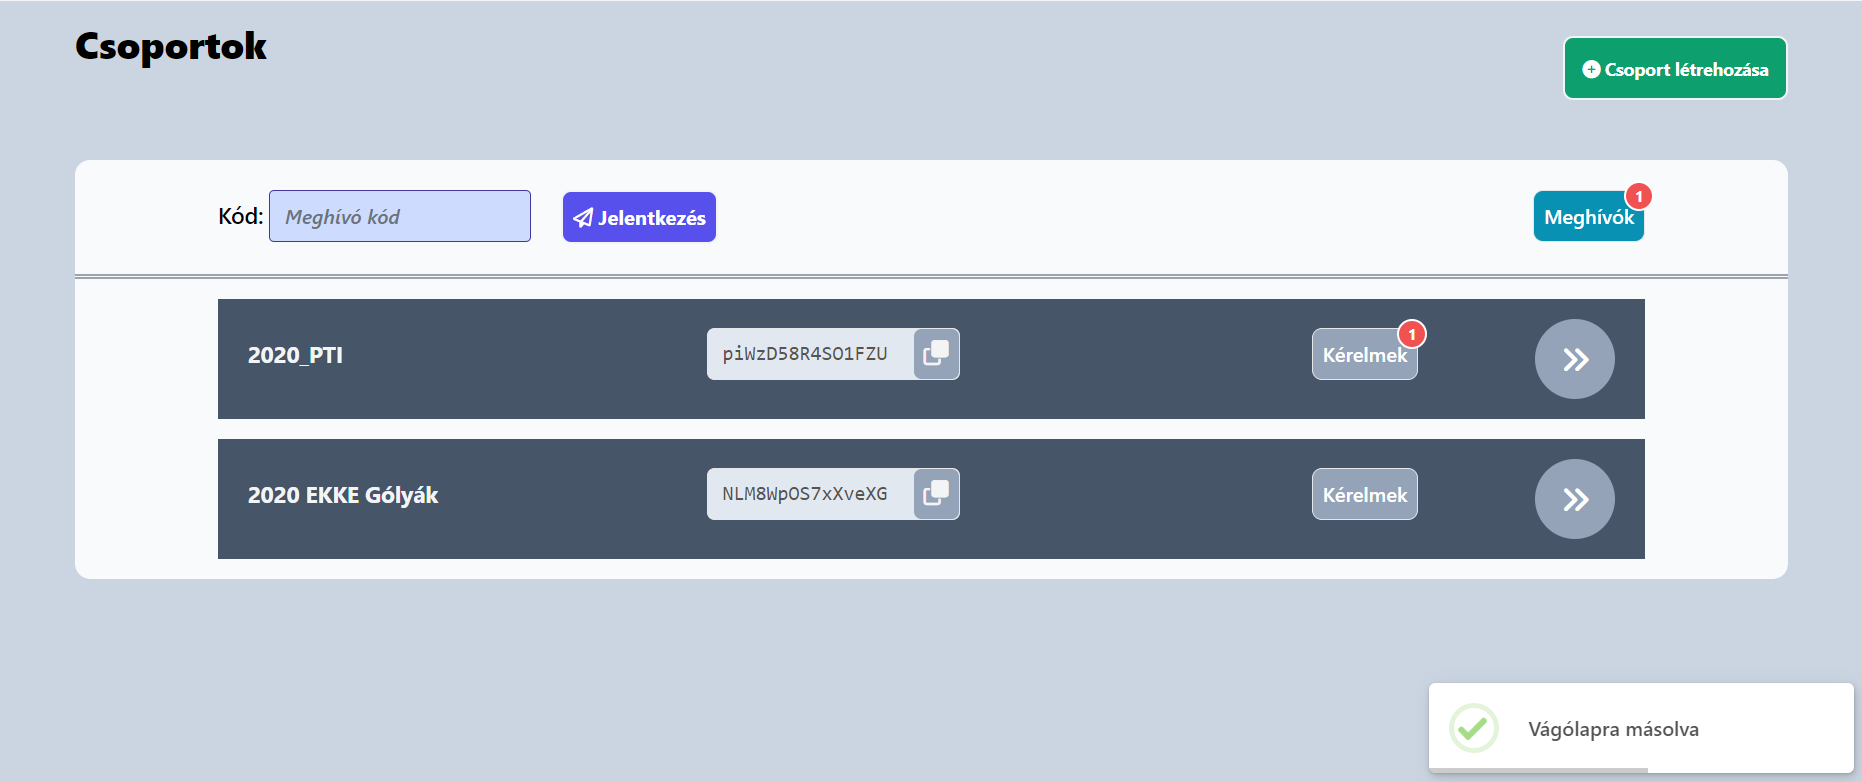
\includegraphics[width=15cm]{Groups.index.png}
                    \caption{A csoportjainkat listázó oldalról képrenyőkép}
    		        \label{fig-csoportok-index}
    	    \end{figure}
                Ahhoz, hogy egy felhasználó tagja lehessen egy csoportnak, két lehetőség áll rendelkezésre:
                \begin{itemize}
                    \item Minden csoport létrehozásakor generálodik egy egyedi, 15 karakter hosszúságú kód, amely állhat számokból illetve kis- és nagykapitális betűkből. Ennek a kódnak a kimásolásához minden olyan csoporthoz biztosítottam egy gombot, amelynek tagjai vagyunk, ezáltal ismerősöket is meghívhatunk a közösségünkbe. A jelentkezés elküldéséhez csupán annyi a teendőnk, hogy a csoportok főoldalán található beviteli mezőbe beillesztjük a kimásolt kódot, majd elküldjük a csatlakozási kérelmünket. 

                    Minden csoport adminisztrátorának (aki létrehozta azt) látható egy-egy gomb ,,Kérelmek'' felirattal. Itt láthatjuk a jobb felső sarkában, hogy jelenleg hány jelentkezési kérelmünk várakozik elbírálásra a csoporthoz.

                    Erre kattintva kilistázhatjuk az összes jelentkezni kívánt felhasználót, ahol eldönthetjük, hogy elfogadjuk vagy elutasítjuk a kérelmet

                    \begin{figure}[ht!]
    		        \centering
    		        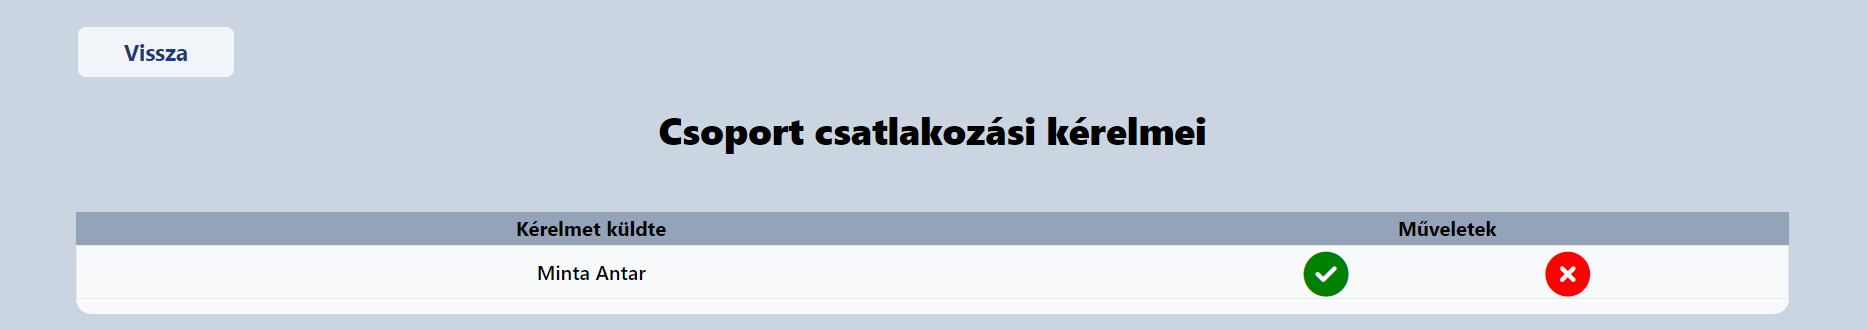
\includegraphics[width=15cm]{Groups.join.requests.png}
                        \caption{Kép egy csoport csatlakozási kérelmeit listázó oldalról}
    		        \label{fig-groups-joinrequests}
    	        \end{figure}

                    \item Amennyiben mi hoztuk létre a csoportot, az online dokumentációban\cite{Livewire-Search} található módon létrehozott Livewire kereső komponens segítségével kereshetünk e-mail cím szerint a létrehozott felhasználók között. Abban az esetben, ha a megadott e-mail címre kapunk találatot, kislistázzuk, majd kattintással kijelölhetjük. Ilyenkor a kereső mező alatt megjelenik a kijelölt elemnek egy kis kártyája. Akár több felhasználót is kijelölhetünk egyszerre. A kérelmek kiküldéséhez a ,,Meghívás'' gombra kell kattintanunk, amely során átküldjük a szerver felé, ahol rögzítünk a felhasználókhoz 1-1 meghívót a csoportunkba. Ebben az esetben szintén a főoldal jobb felső sarkában található ,,Meghívók'' gombra kattintva találhatjuk meg ezeket a meghívási kérelmeket. Ez majdnem teljesen olyan, mint a csatlakozási kérelmek oldala, viszont itt azt is látjuk, hogy mi a csoport neve, amelybe meginvitáltak minket.
                    \begin{figure}[ht!]
    		        \centering
    		        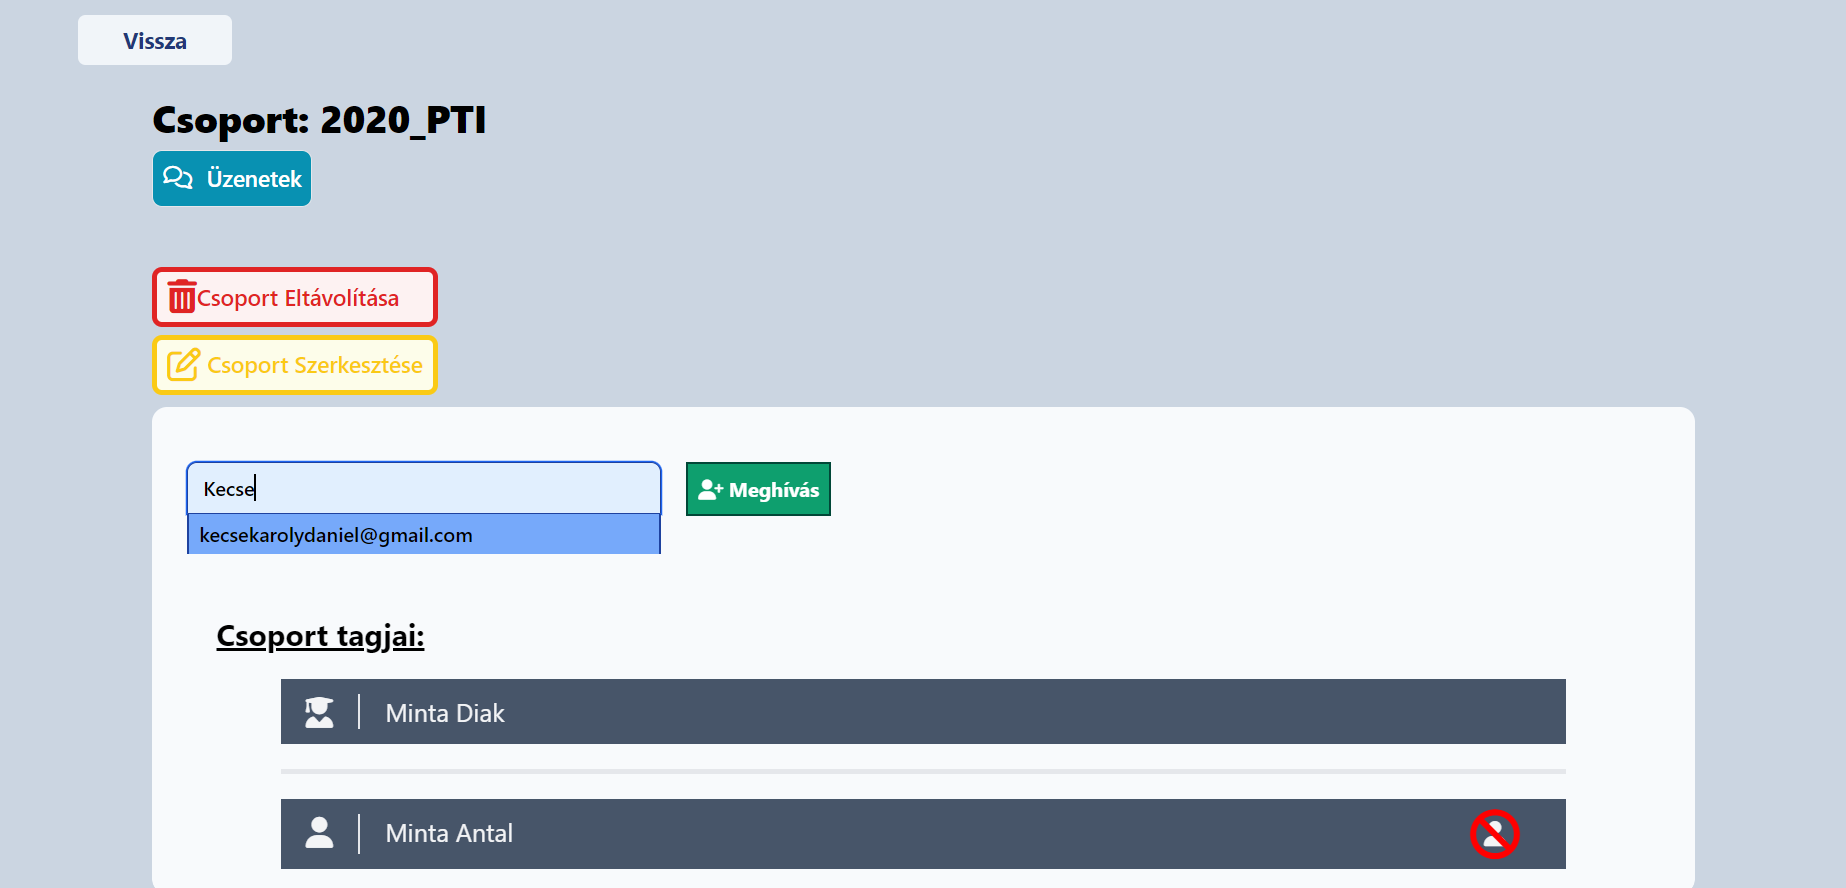
\includegraphics[width=15cm]{Groups.show.png}
                        \caption{Egy csoport kiválasztásánál kapott oldal}
    		        \label{fig-csoportok-show}
    	        \end{figure}
                    
                \end{itemize}
            \section{Felhasználók eltávolítása a csoportjainkból}
                Amennyiben a csoport adminisztrátora távolít el minket valamilyen oknál fogva a csoportból, kapunk egy értesítést az e-mail címünkre, amelyben láthatják, hogy mely csoportból lettek kirúgva.

                Másik lehetőség, hogy a felhasználó saját maga lép ki a csoportból, ilyenkor nem kap senki üzenetet.
                
            \section{Chat: Pusher és Echo}    
                A chat felületét minden olyan felhasználó elérheti -- aki tagja a csoportunknak -- az ,,Üzenetek'' gombra kattintva. Ekkor megjelenik az alábbi felület:
                \begin{figure}[ht!]
    		    \centering
    		    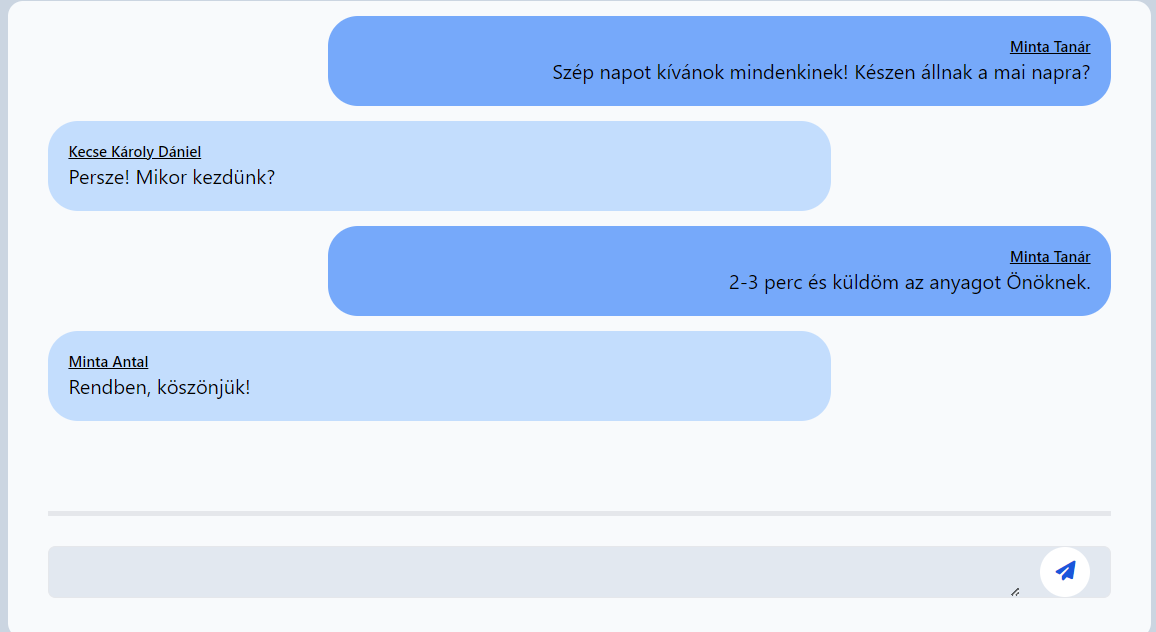
\includegraphics[width=15cm]{Group.chat.png}
                    \caption{Példa egy csoportos csevegésről}
    		    \label{fig-csoportok-chat}
    	    \end{figure}

                Mivel egy alap elvárás egy ilyen funkciónál, hogy a felhasználóknak ne kelljen mindig frissíteni az oldalt, hogy megnézzék, küldött-e valaki egy új üzenetet, ezért valami WebSocket-hez hasonló megoldást kellett keresnem. Mivel nem voltam járatos a témában, ezért további alternatívák felé kutattam és megtaláltam a Laravel által ajánlott Broadcastingot. Két JavaScript-en alapuló package segítségével biztosítottam, hogy a szerver oldalon kiváltott eseményt figyelni tudjam a kliens oldalon is egy meghatározott csatornán, ahol le tudom reagálni az egyes változásokat. 

                Ennek a működése a következő képpen történik nagy vonalakban:
                A felhasználók a felületen feliratkoznak egy adott csatornára, majd ebbe a csatornába küldjük a backend egyes eseményeit, amit a kliens oldalon feldolgozunk. 

                A szerveroldali üzenet broadcastolásához használtam a \emph{Pusher-Channels}\cite{Pusher-Channels} csomagot. Ennek használatához egy-egy üzenet létrehozása után elindítok egy broadcast-ot, aminek átadok egy eseményt, amelyet felparamétereztem a csoport azonosítójával. Ezen az eventen belül pedig egy ,,\emph{broadcastOn()}'' metódusban létrehozok egy új privát csatornát, amelynek a neve ,,groupMessagesX'', ahol X a csoport ID-je, értesítve ezzel a csatorna többi tagját, hogy egy új üzenet került elküldésre és ezt le kellene kérdezniük.

                Erre a csatornára a kliens oldalon a \emph{Laravel-Echo}\cite{Laravel-Echo} package segítségével feliratkozunk úgy, hogy megadjuk, hogy milyen csatornára szeretnénk ,,ráállni'' és azon belül is milyen eseményt figyelünk. Amennyiben kiváltásra került az event, indítunk egy GET-es kérést a szerver felé, ahol lekérdezzük a csoportunkba legutoljára felvitt üzenet szövegét, amit megjelenítünk a Livewire komponensünk segítségével.
                
        \chapter{A kurzosok bemutatása}\label{Kurzusok-bemutat}
            A projekt kurzusai szolgálnak az egyes tanórák gyűjtő egységének. Lehetősége van a kurzus tulajdonosának felhasználókat és csoportokat hozzárendelni a kurzusokhoz, valamint tananyagoknak (moduloknak) a létrehozásához. Készíthetnek kvízeket, amelyeket vagy magához a kurzushoz, vagy egy-egy modulhoz kapcsolnak. A jegyszerzés biztosításához pedig készíthetnek vizsga feladatsorokat, amiket egy megadott indőintervallumban kitölthetnek a tanulóink.

            Minden olyan kurzushoz hozzáférhetünk, amihez vagy személyesen, vagy csoporton keresztül el kellene tudnunk érni. A tagok hozzárendelésénél ugyanaz a Livewire komponens került felhasználásra, amely végzi a felhasználók csoportokhoz rendelését. A képernyőképen látható gombok megjelenítése és működése itt is a policy-k segítségével valósul meg.
            \begin{figure}[ht!]
    		\centering
    		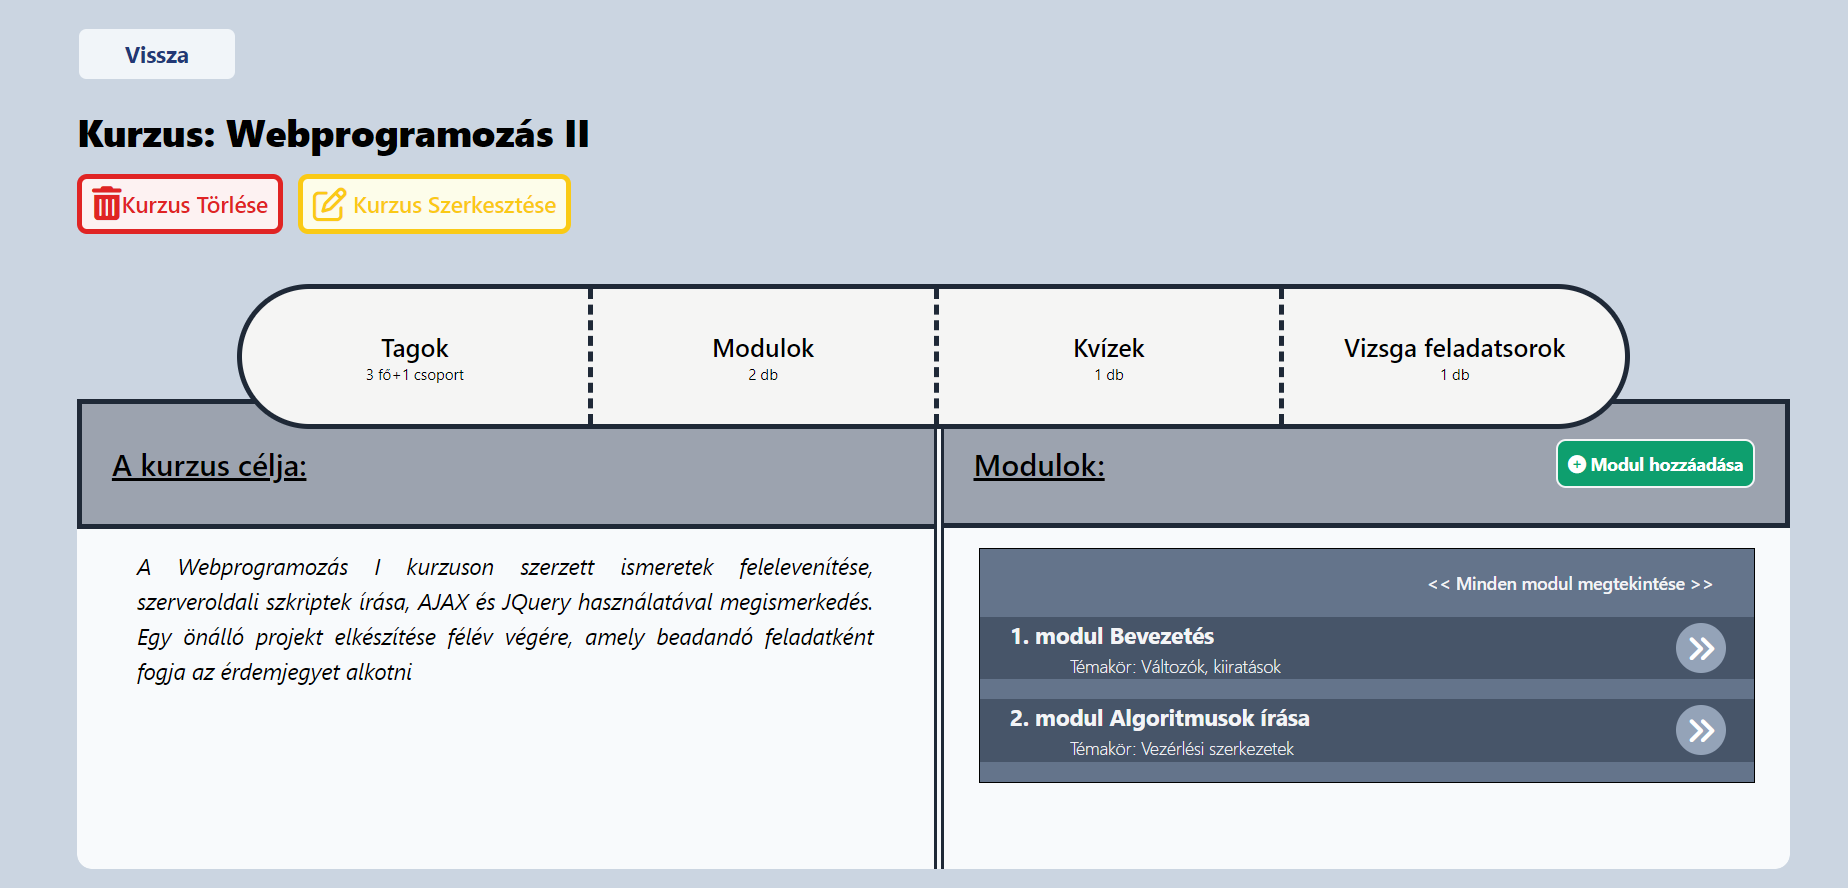
\includegraphics[width=15cm]{Courses.show.png}
                \caption{Egy kurzus megtekintésénél ez az oldal fogad minket}
    		\label{fig-kurzusok-show}
    	\end{figure}
     
            \section{Modulok}
            Ezek az egységek tartalmazzák a kurzusok tananyagait. Itt egy TinyMCE felület található, amely biztosítja az összes olyan alapvető eszközt, amely a tananyag megírásához és összeállításához szükséges lehet.
            
            A szerkesztő felület abban az esetben jelenik meg, ha a kurzus tulajdonosa (tehát a tanár) létrehozásra vagy szerkesztésre nyitja meg a modult. Ilyenkor módosíthatja a témakört, az óra megnevezését illetve a tananyag tartalmának szövegét.
                \begin{figure}[ht!]
    		        \centering
    		        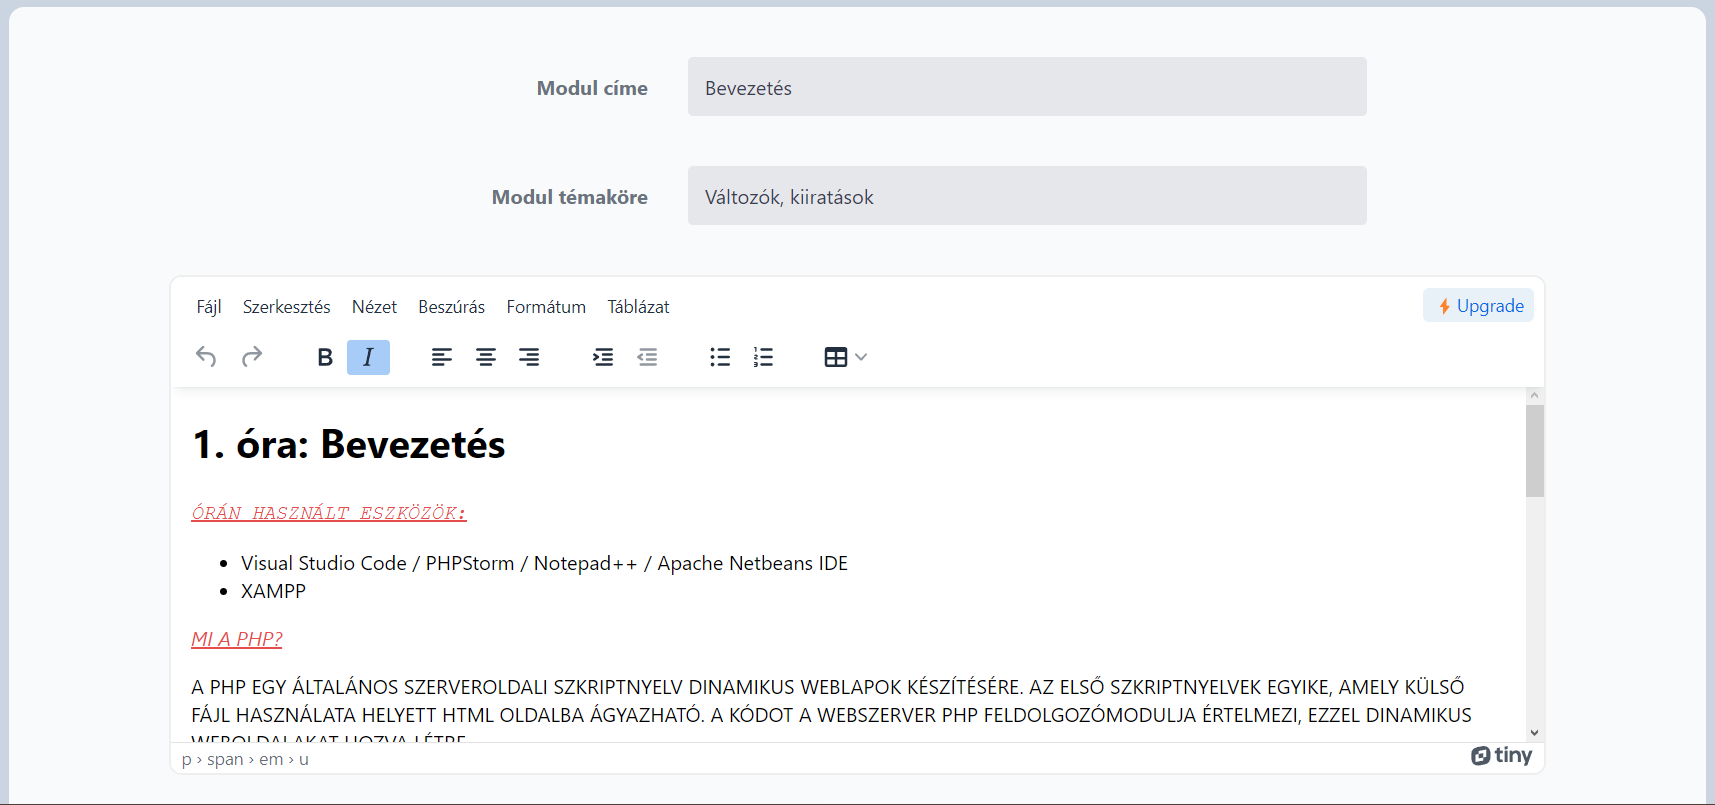
\includegraphics[width=15cm]{Modules.edit.png}
                        \caption{Egy adott modul tananyagának szerkesztése}
    		        \label{fig-modulok-edit}
    	    \end{figure}
                \begin{figure}[ht!]
    		        \centering
    		        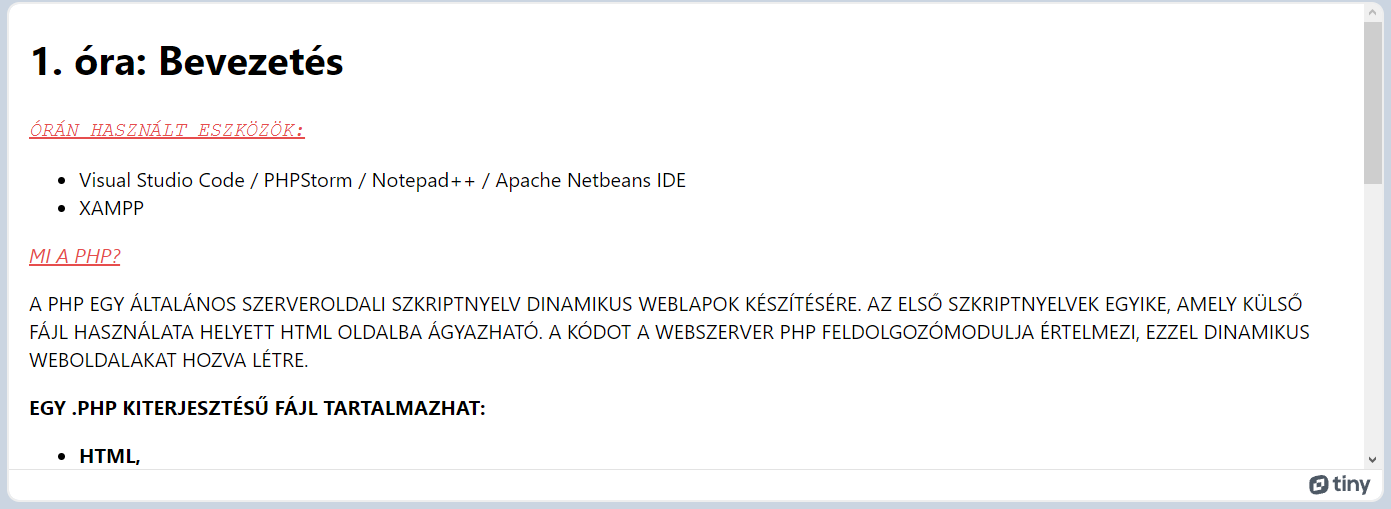
\includegraphics[width=15cm]{Modules.show.png}
                        \caption{Egy adott modul tananyagának megtekintése}
    		        \label{fig-modulok-show}
    	    \end{figure}

            A tananyag egésze egy ,,textarea''-ban van eltárolva, ennek az értékét fogjuk eltárolni egy ,,blob'' típusú mezőben az adatbázisunkban. Ez tartalmaz minden, a tananyagot képező HTML taget, annak osztályát és inline CSS beállítását. Azért, hogy ezek megfelelően jelenjenek meg az oldalon a megtekintés során, ugyanolyan szerkesztőfelületbe töltjük bele a ,,material'' mező értékét, mintha szerkesztenénk, viszont readonly módban nyitjuk meg és a szerkesztői fejlécet eltüntetjük.
            
        \chapter{A tesztek felépítése és kitöltése}\label{Tesztek-bemutat}
            A projektben található tesztek segítségével tudjuk biztosítani, hogy a tanulók visszacsatolást szerezzenek -- kvízek segítségével -- a jelenlegi tudásukról, illetve, hogy számot adjanak arról -- vizsga feladatsorok kitöltésével --, hogy mennyire tudták elsajátítani az egyes kurzusokhoz tartozó tananyagot.

            A tesztek létrehozásához és szerkesztéséhez 1-1 Livewire komponens került elkészítésre. Ezeknek a használatakor elkülönül az oldalak működése oly módon, hogy ha tudjuk, hogy kvízt készítünk, letiltunk (Kitöltések száma, kitöltésre szánt idő megadása) illetve hozzáadunk (Modul kiválasztása) néhány funkciót, míg vizsga feladatsor összeállításánál ennek a fordítottját hajtjuk végre. 
            
            Ezt a létrehozásnál úgy tudjuk megtenni, hogy a komponens hívásakor egy paraméterben átadom a teszt típusát, szerkesztésnél pedig a komponensnek átadott teszt típusa alapján tudjuk, hogy mivel is kell majd dolgoznunk a feldolgozás során.
      
            \section{Service-ek}
            Annak érdekében, hogy a teszteket a Livewire komponenseimen belül megfelelően tudjam kezelni, szükséges volt egy hosszadalmasabb átalakítása a modelljeimnek. Emiatt szükségessé vált, hogy kiszervezzem a meglévő metódusaim bizonyos részleteit egy külön osztályba/osztályokba, hiszen túlságosan hosszúvá váltak a kontrollerjeim ahhoz, hogy átlátható és tiszta legyen a kód.

            Mivel minden ilyen blokk a ,,Test'' modellen végzett valamilyen műveletet, ezért úgy döntöttem, hogy az ,,Action'', ,,Job'' és ,,Service'' osztályok közül inkább az utóbbit választom. Amíg az előző két osztály lényegében 1-1 metódus elvégzésére használatosak, addig a Service-be elhelyezhetek több, logikailag összetartozó metódust. 
            
            Ebbe a ,,TestService'' osztályba tartoznak azok az eljárások és függvények, amelyek elvégzik a tömb adatszerkezetben eltárolt tesztjeim mentését illetve módosítását, valamint a megkapott ,,Test Model'' (és az ahhoz tartozó kapcsolatok) átalakítását szintén tömb adatszerkezetté, így megkönnyítve a későbbi data bindingot illetve a megjelenítést.

            \section{Feladatlapok megvalósítása}
            \begin{figure}[ht!]
    		\centering
    		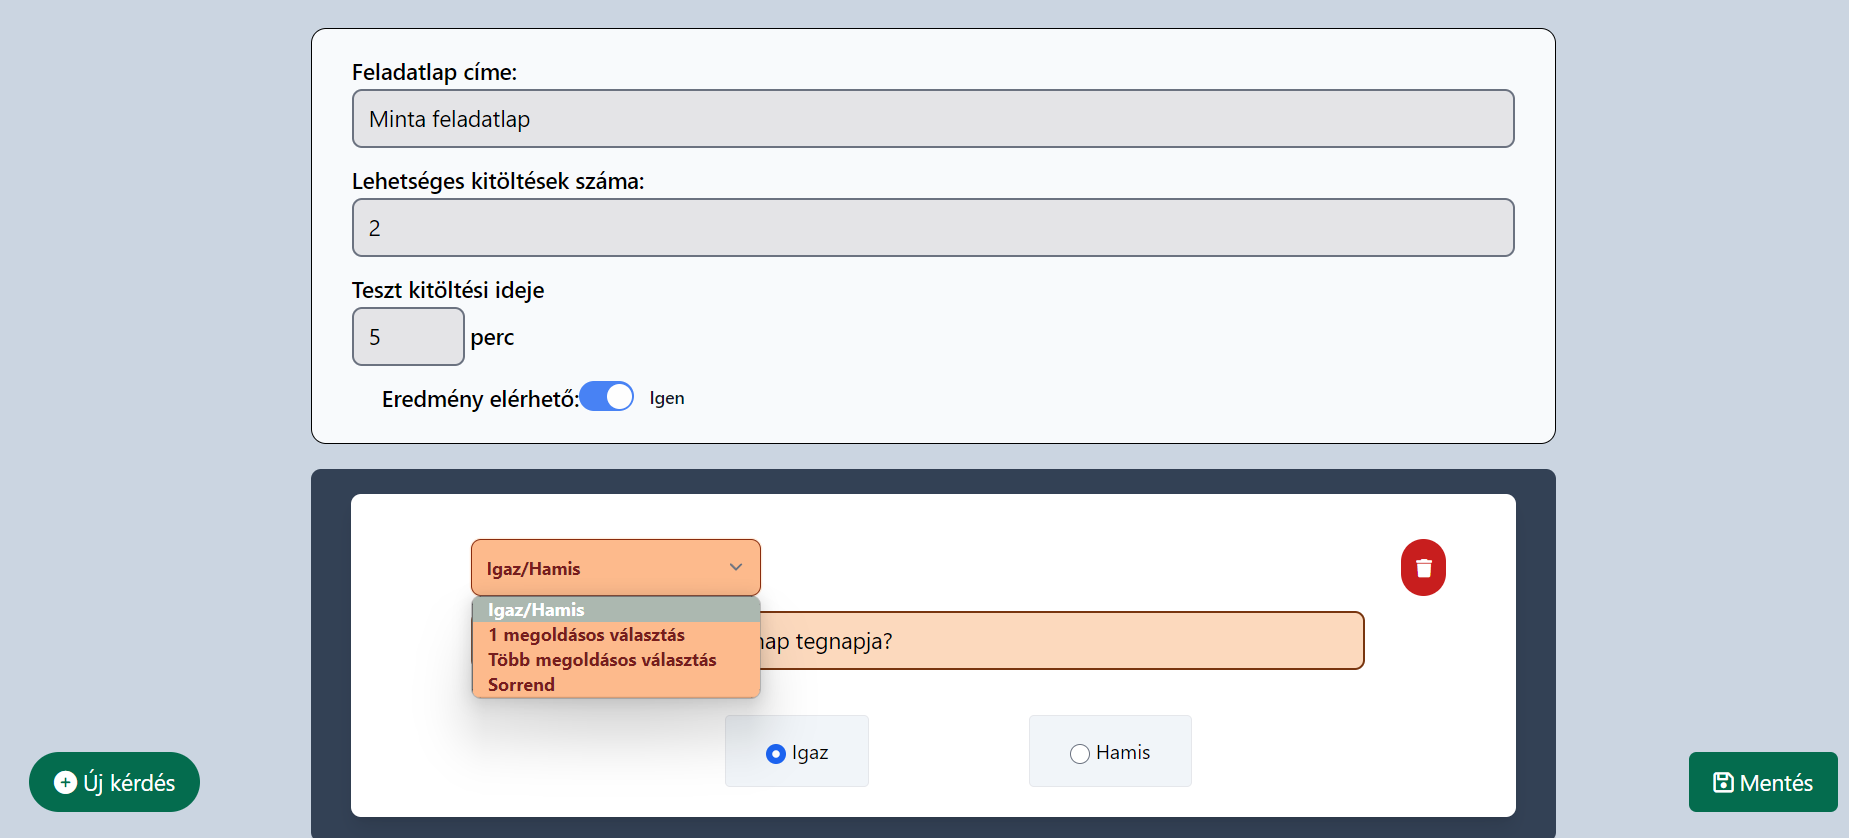
\includegraphics[width=15cm]{Test.create.png}
                \caption{Egy vizsga feladatsor létrehozása}
    		\label{fig-tesztek-create}
    	\end{figure}
            Miután a teszt fejlécét kitöltöttük, fel kell töltenünk a tesztünket tartalommal, aminek az elvégzéséhez található a bal alsó sarokban egy ,,Új kérdés'' feliratú gomb.
            
            Egy kérdés hozzáadása után meg kell adnunk, hogy milyen legyen a típusa. Itt 4 lehetőség közül választhatunk -- Igaz/Hamis, Egy-, Több lehetséges megoldás kiválasztása, Sorrend) --, ahol egy opció kijelölése után ,,emitelünk'' egy eseményt a Livewire backend felé, ahol ezt figyeljük egy ,,listener'' segítségével, majd az alábbiakat tesszük: 
            \begin{itemize}
                \item Ha a kiválasztott típus \emph{Igaz/Hamis}, az adott kérdéshez kapunk két választási lehetőséget. Ezek az ,,Igaz'' és ,,Hamis'' feliratot kapják. Itt rá kell kattintanunk arra, amelyet a kérdés megoldásának szánunk.
                \item Minden egyéb esetben nekünk kell újabb válaszlehetőséget rendelnünk a kérdéshez, ahol megadjuk a legalább 5 karakter hosszúságú feliratát, majd itt is kijelöljük a helyes megoldásokat, vagy megfelelő sorrendbe állítjuk őket abban az esetben, ha sorrend típusú feladatról beszélünk. 
            \end{itemize}

            A dinamikus hozzáadáshoz, törléshez, a szövegek eltárolásához és a helyes megoldások kijelöléséhez a már korábban emlegetett \emph{data-binding}-ot és \emph{action}-t használjuk úgy, hogy a \ref{Test-structure}.~bekezdésben említett struktúrának megfeleljünk.

            Minden egyes kérdéshez tartozik egy szöveg, típus, válaszlehetőségek tömbje illetve az \emph{Igaz/Hamis} és  az\emph{Egy megoldásos} feladattípusok megoldásainak eltárolásához egy ,,right\_option\_index'' kulcs-érték pár. Ilyenkor a kérdések megoldásainak eltárolásá miatt a ,,right\_option\_index''-en belül eltároljuk annak a válaszlehetőségnek az index-ét, amelyet a felhasználó helyes megoldásként jelölt meg.

            Minden válaszlehetőség egy szövegből, pontszámból és egy ,,solution'' kulcs-érték párból áll. A pontszám abban az esetben lesz 1, amennyiben az helyes megoldásként van megjelölve a feladatlap elkészítése során. A ,,solution''-be kerül eltárolásra, hogy az adott opció helyes megoldásként van-e megjelölve, vagy sem. Ezt kulcsot a \emph{Sorrend} és a \emph{Több megoldásos} feladatoknál használjuk fel úgy, hogy a checkbox-okat és diveket az adott opció ,,solution'' kulcsához rendeljük. Ez abban az esetben kap értéket, ha a felhasználó bepipálja azt a \emph{Több megoldásos} feladatnál az adott választ, a \emph{Sorrend} kérdéseknél pedig automatikusan a sorban elfoglalt indexét kapja.

             Amikor egy-egy gombra kattintunk, legyen az törlést vagy hozzáadást végrehajtó, mindig egy ,,wire:click'' action-t hívunk meg, aminek határása lefut egy-egy eljárás. Ezek a függvények biztosítják az alábbi műveleteket:
            \begin{itemize}
                \item a kérdés hozzáadását: a ,,\emph{\$questions}'' array-hez ad hozzá egy elemet,
                \item a kérdés eltávolítását: a ,,\emph{\$questions}'' array-ből eltávolítja a paraméterből érkező ,,\emph{\$questionIndex}''-edik elemet,

                \item opció hozzáadását: a ,,\emph{\$questions}'' tömbnek a paraméterből érkező ,,\emph{\$questionIndex}''-edik elemének ,,\emph{\$options}'' tömbjéhez ad egy elemet,
                \item opció eltávolítását: a ,,\emph{\$questions}'' tömbnek a paraméterből érkező ,,\emph{\$questionIndex}''-edik elemének ,,\emph{\$options}'' tömbjének ,,\emph{\$optionIndex}''-edik elemét távolítja el,
                
                \item teszt mentését: létrehozok a fejlécben megadott adatokkal egy ,,\emph{Test}'' modellt, majd azt átadom a \emph{TestService} \emph{store} metódusának az eltárol ,,\emph{\$questions}'' tömbbel együtt.
            \end{itemize}
            
            \section{Teszt kitöltésének folyamata}
                 Amennyiben egy adott kurzus tesztjét szeretnénk kitölteni, először is kötelezően tagnak kell lennünk, egyébként a Policy miatt nem fogunk tudni hozzáférni. Ezután a \emph{TestService} ,,getTestToWrite'' függvényével átalakítjuk tömb adatstruktúrává a Test modellünket minden relációjával együtt, majd ezt átadjuk a kitöltést elvégző Livewire komponensünknek.
                \subsection{Kvízek}
                    A teszt létrehozásánál tárgyalt módon történik itt is az adatoknak az összeköttetése, viszont itt eltároljuk a helyes válaszok indexét is, hiszen ebben az esetben nem probléma, ha valahogy kiderülne, hogy mik a helyes megoldások. A teszt kitöltése után megtekinthetik a megadott válaszaik eredményét, illetve újra megpróbálkozhatnak a kitöltéssel, amennyiben nem elégedettek a teljesítményükkel. Ebben az esetben az összes kérdést, illetve az \emph{Igaz/Hamis} típusú feladatok kivételével az összes válaszlehetőséget is összekeverjük, majd megjelenítjük ismételten a kvízt. Itt fontos, hogy a próbálkozások eredményei nem mentődnek, illetve akárhányszor kitölthető tetszőleges időn keresztül, korlátozások nélkül.
                \subsection{Vizsgák}
                    Vizsgák esetén azon a feltételen felül, hogy kurzus tagnak kell lennünk, van egy másik korlátozás is. A kurzus tulajdonosa megadhatja, hogy a vizsga feladatsorok a diákok számára milyen időintervallumban lehessenek elérhetőek. Ennek megfelelően egy kissé összetettebb policy-n is át kell esniük a felhasználóknak, amely ellenőrzi, hogy jogosult-e a kurzushoz, elérhető-e a jelenlegi dátumon a teszt kitöltése, és van-e még további kitöltésre lehetőségünk. Mivel a vizsga feladatsorok csak korlátozott számmal tölthetőek ki, ezért előfordulhat, hogy kifutunk a próbálkozásokból.

                    Amennyiben biztosak vagyunk abban, hogy elindítjuk a teszt kitöltését, rögzítünk egy ,,testAttempt'' rekordot, amellyel jelzezzük, hogy van egy aktív próbálkozása az adott diáknak egy adott teszthez. Ilyenkor ezzel egy időben egy \emph{Queued Job}-ot is indítunk, amely biztosítja azt, hogy egy próbálkozást akkor is lezárunk, ha a diák valamilyen oknál fogva kilépne a rendszerből. 
                    
                    Azért, hogy ne keveredjenek össze a szálak, egy minimális időeltolást alkalmazunk. Ha van egy teszt, aminek a kitöltésére 5 percünk van, akkor ezt a Job-ot 5 perc és 1 másodperccel időzítem, hiszen amennyiben a diák felhasználja mind az 5 percet, amely a rendelkezésére áll, akkor a rendszer automatikusan lezárja a kitöltést, majd ezután a beérkező Job észreveszi, hogy a próbálkozást lezáruk és be is fejeződik. 
                    Amennyiben mindketten azonosan 5 perc után hajtódnának végre, előfordulhatna az, hogy érvénytelen próbálkozásnak veszi a Job miatt és nem kerülne kiértékelésre a dolgozat.

                    Annak érdekében, hogy eltároljuk a teszt kitöltésének előrehaladását, a vizsga megkezdésekor az összeállított teszt tömbjét eltárolom a session-ben a kezdés időpontjával együtt (ebből is kiszámolhatom a hátralévő időt) a próbálkozás azonosítójának segítségével.

                    Amikor megpróbálkozunk a vizsga kitöltésével, megnézzük, hogy van-e az adott felhasználónak egy már megnyitott, de be nem fejezett próbálkozása az adott teszthez. Ha van, kiolvassuk az adott ID-vel eltárolt session változóból, viszont amennyiben ez nem található, sajnos elveszett az elmentett adat, ezért egy újabb Service hívással összeállítunk egy tesztet és megkezdődik elölről a kitöltés a hátralévő idővel.
                    
                    A teszt kitöltése alatt 5 másodpercenként felülíródik az eddig eltárolt előrehaladás a munkameneten belül. Ezt a ,,\emph{wire:poll.5s="SaveDataToSession"}''-nel tudjuk elvégezni, amely 5 másodpercenként meghívja a megadott eljárásom.
                    
                    \begin{figure}[ht!]
    		        \centering
    		        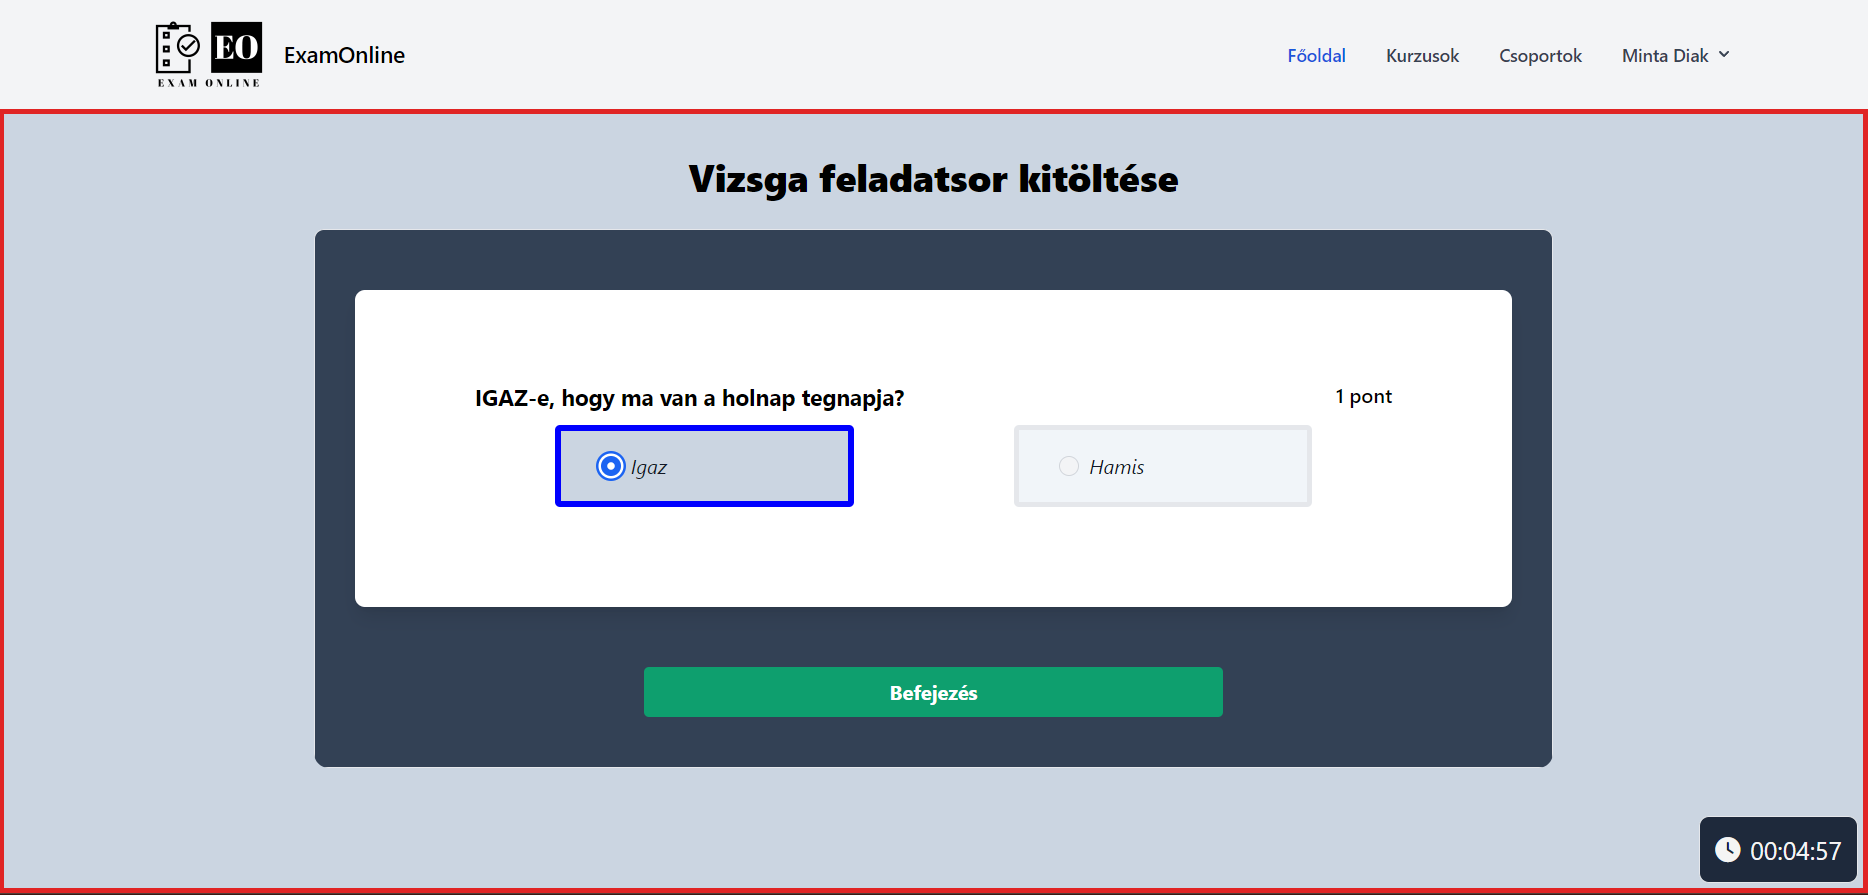
\includegraphics[width=15cm]{Test.write.png}
                        \caption{Egy vizsga feladatsor kitöltésére példa}
    		        \label{fig-teszt-write}
    	           \end{figure}
                
                    A teszt kitöltése közben látható egy számláló ahol láthatjuk még rendelkezésre álló időnket, illetve egy vörös keretet a teszt körül. Amennyiben a kitöltő kurzora 1 másodpercnél tovább marad kint a megengedett tartományon kívül, a tesztre visszahúzva a kurzorát befejeződik a kitöltés és kiértékelődik a tesztje az eddigi megadott válaszai alapján.
                    
                    Mivel az online oktatás során megtanultam, hogy a diákok bármire képesek annak érdekében, hogy megkönnyítsék a digitális számonkérést, tudom, hogy ez sem teljes megoldás, viszont megpróbálkoztam az egyértelmű csalásokat kiszűrni.
        \chapter{Az alkalmazás tesztelése}
            A projekt tesztelésére kiemelt hangsúlyt fektettem az alkalmazás fejlesztése során, hiszen mindenképpen egy teljesen jól funkcionáló, hibáktól mentes rendszert akartam kiadni a kezeim közül. Az egyes funckiók elkészítése után mindig elvégeztem egy, vagy több ahhoz tartozó manuális tesztet. Csak abban az esetben léptem át egy következő fejlesztési folyamatra, amennyiben az általam elvárt eredményeket sikerült produkálnia a rendszernek.

            Az alkalmazás növekedésével egyre több időbe telt, hogy az oldal egészét leteszteljem, ezért szükség volt egy automatizálható tesztre. Mivel sok jót hallottam a Cypressről, ezért úgy döntöttem, hogy ezt fogom használni a továbbiak során. A legtöbb funkciót így sikerült letesztelnem, viszont a feladatsorok kitöltését mindeképpen manuálisan kell még mindig tesztelni, hiszen minden egyes feladatlap más sorrendben generálja a kérdéseket és az azokhoz tartozó válaszlehetőségeket.

            A Cypress egy nyílt forráskódú, JavaSript nyelven íródott keretrendszer, amely segítségével automatizált teszteket végezhetünk el a fontendünkön végezhető műveleteken. Az egyik legnagyobb előnye, hogy könnyen és gyorsan tesztelhetjük a rendszerünket úgy, hogy a tesztelő integrálása is egyszerűen megoldható.

            A Laracasts Cypress GitHub\cite{LaracastsCypress} oldalán található telepítési útmutatóval néhány perc alatt elérhetjük, hogy használhassuk a rendszerünkön belül. Az általuk készített Youtube videó\cite{LaracastsCypressYoutube} segítségével készültek el a projekt egyes tesztjei.

            Szinte minden teszt az alábbi utasításokat tartalmazza:
            \begin{itemize}
                \item ,,\emph{cy.login(\{username: '...'\})}'': bejelentkezünk a rendszerbe egy olyan felhasználóval, akinek a felhasználóneve a paraméterben megadott értéknek megfelel. Amennyiben létezik már ilyen értékű mezővel rekord, azzal belépünk, egyéb esetben a paraméterben meghatározott értékekkel létrehozunk egy rekordot, majd azzal bejelentkezünk. Az utóbbi esetben a meg nem határozott, kötelezően kitöltendő mezőknek véletlenszerűen generált értékeket ad a keretrendszer.
                \item ,,\emph{cy.visit('...')}'': a paraméterben meghatározott útvonalra navigál. Az itt található elemkre írhatunk DOM-os vizsgálatokat, amikhez a következő 2 pontban leírtakat használtam.
                \item ,,\emph{cy.get('...')}'': paraméterben megadunk DOM kijelölőket, mint például HTML tag típusa, osztály vagy azonosító.
                \item ,,\emph{cy.contains('...')}'': a paraméterben megadott szöveggel keresünk az oldalon egy elemet.
                \item Amennyiben a kijelölt elemünk egy gomb, a ,,\empty{click}'' metódust meghívhatjuk. Ezzel szimuláljuk az elemre kattintást. Ha egy szöveges mezőnek szeretnénk értéket adni, a ,,\emph{type}'' eljárást használjuk, aminek paraméterének meg kell adnunk, hogy mit helyezzünk el az adott beviteli mezőben. Egyéb input tageken végezhető eljárások a ,,\emph{check}'' és  a,,\emph{select('select\_option\_szovege')}''.
            \end{itemize}
            Az ,,\emph{npx cypress open}'' parancs kiadása után az E2E (End To End) teszt és a böngésző kiválasztása után meg kell adnunk, hogy melyik az a teszt fájlt, amit szeretnék futtatni. Ezután láthatjuk a tesztelő által végrehajtott lépéseket.

            A \ref{CypressTestExample}.~kódban látható egy Cypress tesztre példa. Bejelentkezek egy már létrehozott, ,,mintamarton'' nevű felhasználóval és létrehozok egy új csoportot, majd vizsgálom, hogy visszakapom-e a megerősítő üzenetet az oldalon.
            \lstinputlisting[caption=Cypress példa csoport létrehozásához, label=CypressTestExample]{Cypress\_test\_example.cy.js}
        \chapter{Külső komponensek, technológiák}\label{Kulso}
            \section{SweetAlert}
            	A SweetAlert egy rendkívül elterjedt JavaScript könyvtár, amely segítségével felugró ablakban üzenhetünk a felhasználónak. Számos konfigurációs lehetőség áll rendelkezésünkre, ahol többek között a megjelenített szöveg témájához tudjuk igazítani az ablakban megjelenő animációt, ikont illetve gombokat. Megadhatjuk, hogy hogyan viszonyuljon az oldal többi eleméhez (ne engedje a usert kikattintani belőle). 
            	
            	Kétféleképpen szerepel a projektben, a Laravel-ből\cite{SweetAlert-Laravel} kiváltott ablakok a composer-en keresztül kerültek telepítésre package formájában, a JavaScript-beli használatát pedig egy CDN-es\cite{SweetAlert-js} hivatkozás segítségével biztosítottam.
            	
            	Laravel-ben annyi a feladatunk a használata során, hogy behivatkozzuk a ,,\emph{RealRashid\textbackslash Facades\textbackslash SweetAlert}'' névtérben található ,,\emph{Alert}'' osztályt, majd ennek hívjuk a statikus metódusait. Ezek közül kettőt használtam: a,,\emph{success}''-t és a ,,\emph{warning}''-ot. Egy használat így néz ki: ,,\emph{Alert::success("Sikeres módosítás!");}''. 
            	
            	JavaScript-ben legfőképpen a törlést és frissítést biztosító form-ok elküldésének megerősítésére használtam. Amikor rögzíteni kívánjuk az űrlapunkat, megállítom a küldést, és megjelenítek a Swal.fire metódussal egy felugró ablakot, ahol megerősítés után továbbküldjük a formot, egyéb esetben elvetjük a műveletet.
            \section{Spatie süti engedélyező}
            	A Spatie egy jól ismert szoftverfejlesztő cég, amely nyílt forráskódú csomagokat készít. Széleskörű webfejlesztési problémákra kínálnak megoldást, amikkel általánosságban meggyűlik a bajuk a programozóknak, de ezek akár lehetnek akár gyakran implementálandó funkciók is. 
            	
            	Egy általuk készített package, amit felhasználtam a projekt elkészítése során a ,,\emph{Laravel Cookie Consent}''\cite{Spatie-CookieConsent}, amely kifejezetten a sütik használatának tényének közlésére és elfogadására használatos. Erre azért volt szükséges, mert a teszt kitöltése során a session-be helyezzük el a kitöltött teszt pillanatbeli állapotát. 
            	
            	Ennek a megoldása roppant egyszerű volt, hiszen a csomag telepítése után csak be kellett hivatkozni az oldal tartalma alá az alábbi utasítással ,,\emph{@include("cookie-consent::index")}'', illetve a ,,\emph{.env}'' fájlunkon belüli engedélyezés után csak a megjelenő szöveget kellett személyre szabni.
            	
            \section{TinyMCE}
            	A TinyMCE\cite{TinyMCE} egy olyan nyílt forráskódú, ingyenes WYSIWYG (What You See Is What You Get) szövegszerkesztő, amely biztosítja a felhasználók számára a weboldalakon lévő tartalmak szerkesztését és formázását oly módon, hogy a végrehajtott módosításokat folyamatosan láthatják.
            	
            	Minden olyan funkciót magában hordoz, amelyre szükségünk lehet egy tananyag összeállításához (bekezdések, betűméret, kiemelések, listák használata, táblázatok, Youtube videók beszúrása). Mivel rendkívül könnyű a használata, ezért nem igényel semmi magyarázatot, hiszen nagyon hasonlít a Microsoft Word-ben található funkciók megjelenítéséhez.

                A szerkesztő testreszabásához különböző kiegészítőket telepíthetünk, amelyek kiegészítik az editor funckionalitását, mint például képek, videók beszúrása. A pluginok mellett különféle paraméterezési lehetőségünk is van, mint például a szerkesztői felület csak olvashatóvá tétele, a szerkesztői eszközöket tartalmazó menüsév eltávolítása. Mindezek meghatározására a tinymce inizializációjánál van lehetőségünk. Sajnos az editor ingyenessége miatt a lehetőségeink száma eléggé szűkös, hiszen rengeteg elérhető módosítás fizetős licensz esetében van csak biztosítva. Ezért is az alkalmazásom a legalapvetőbb verziót tartalmazza -- ezért is jelenik meg a jobb felső sarkában az ,,Upgrade'' felirat. 
            	
            	Mivel a szerkesztett szöveget Hypertext-ként tárolja egy \emph{textarea}-n belül, így könnyedén elmenthető adatbázisba, majd ebbe hasonló könnyedséggel vissza is tölthető, biztosítva ezzel a megfelelő megjelenítést. 
            \section{Font Awesome}
                A Font Awesome\cite{FontAwesome} főoldalán az alábbi bemutatkozás található: ,,A Font Awesome az internet az ikonkönyvtára és eszközkészlete, amelyet tervezők, fejlesztők és tartalomgyártók milliói használnak''. Hatalmas választékot kínál vektorgrafikus ikonok körében, amiknek elég nagy része fizetős, viszont az ingyenes kategóriában is egészen biztosan találhatunk számunkra megfelelő elemeket. 

                Az ikonjainkat könnyedén beilleszthetjük egy egyszerű ,,toolkit'' legenerálásával, aminek a \emph{script} hivatkozását kell elhelyeznünk azokon az oldalakon, ahol szeretnénk azokat alkalmazni. Az oldalon kikereshetjük a számunkra megfelelő ikont, majd a számunkra szimpatikus elem kijelölése után egy kattintással kimásolhatjuk annak HTML tagjét, amely tartalmazza azokat a szükséges osztályokat, amelyekkel az oldalon láthatóvá válik. Amellett, hogy igényes megjelenítést ad az oldalunknak, intuitívabbá is tehetjük az oldalunk funkcióit az ilyen ikonok felhelyezésével.

                Az egyszerű használat mellett lehetőség van a szimbólumok személyre szabására is. A megfelelő CSS utasítások segítségével a betűméret, betűszín, valamint a háttérszínt is saját belátásunk szerint módosíthatjuk.
	    \section{Mailtrap}
                A Mailtrap\cite{Mailtrap} egy tökéletes megoldást nyújt az e-mail küldések teszteléséhez egy hamis SMTP szerver biztosításával. Egy felhasználói fiók létrehozása után egyedi kulcsokat (felhasználónév és jelszó) kapunk , amiket a \emph{.env} fájlunkon belül a ,,\emph{MAIL}'' szekció megfelelő részeinek értékül adunk. Eközben ügyeljünk arra, hogy az API azonosítók lekérését ne zárjuk be addig, amíg biztosak nem vagyunk abban, hogy a szerverünk megfelelően működik.

                A helyes konfigurálás után elérhetjük azt, hogy a fejlesztés során elküldendő leveleket ne egy más által esetlegesen használatban lévő e-mail-re küldjük ki, hanem a küldésnek csak a funkcionalitását teszteljük úgy, hogy összes elküldött e-mail-t egyetlen helyen összegyűjtjük, azokat elemezzük és utána elvégezzük az esetleges finomításokat a programunkon.

                A tesztelés során havonta 100 e-mail-t küldhetünk az ingyenes verzióban, így bőven biztosított számunkra, hogy akár több megjelenítést is kipróbáljunk a fejlesztés során.
                \begin{figure}[ht!]
    		    \centering
    		    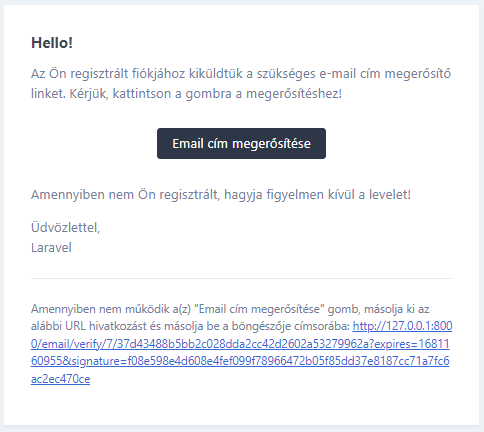
\includegraphics[width=10cm]{Mailtrap_register.png}
                    \caption{Regisztrációt megerősítő e-mail}
    		    \label{fig-mailtrap-register}
    	    \end{figure}
                \begin{figure}[ht!]
        		\centering
    		    
\includegraphics[width=10cm]{Mailtrap_kick.png}
                    \caption{A felhasználót értesítő e-mail arról, hogy eltávolították egy csoportból}
    		      \label{fig-mailtrap-kick}
    	     \end{figure}
        \chapter{Telepítési útmutató}
        Hajtsuk végre az alábbi lépéseket az alkalmazás telepítése során:
        \begin{enumerate}
            \item Töltsük le/klónozzuk a GitHub repository-t!
            \item A konzol felületen navigáljunk el a klónozott/kicsomagolt állományba!
            \item Futtassuk az \emph{\textbf{npm install}} parancsot!
            \item Adjuk ki a \emph{\textbf{composer install}} utasítást!
            \item \emph{\textbf{composer require pusher/pusher-php-server}} és \emph{\textbf{npm install -{}-save-dev laravel-echo pusher-js}} utasításokkal telepítsük az üzenetek küldéséhez szükséges csomagokat!
            \item Generáljuk le az alkalmazás egyedi kulcsát a \emph{\textbf{php artisan key:generate}}-tel!
            \item A ,,\emph{.env.example}'' fájlnak megfelelően \textbf{készítsünk egy új fájlt \emph{.env} névvel}!
            \item Az \textbf{APP\_URL} értéke legyen a következő: \textbf{http://localhost:8000}!
            \item Az adatbázis beállításokat a saját adatbázisunknak megfelelően írjuk át!
            \item A \textbf{BROADCAST\_DRIVER} értékét írjuk át ,,\emph{log}''-ről ,,\emph{\textbf{pusher}}''-re!
            \item Adjuk hozzá az alábbi sort a Laravel Debugbar kikapcsolásához: \textbf{DEBUGBAR\_ENABLED=false}!
            \item A \textbf{QUEUE\_CONNECTION} értékét írjuk át ,,\emph{sync}''-ről ,,\emph{\textbf{database}}''-re!
            \item A ,,MAIL'' szekció beállításait konfiguráljuk az SMTP szererünknek megfelelően. Amennyiben Mailtrap-et szeretnénk használni tesztelés miatt, a \textbf{MAIL\_HOST}-ot  írjuk át ,,\emph{\textbf{sandbox.smtp.mailtrap.io}}''-re, a \textbf{MAIL\_PORT}-ot ,,\emph{\textbf{2525}}''-re, a \textbf{MAIL\_ENCRYPTION}-t ,,\emph{\textbf{tls}}''-re. Ezután hozzunk létre egy fiókot a \url{https://mailtrap.io}-n, majd a \url{https://mailtrap.io/api-tokens} oldalon generáljunk le egy API kulcsot. A \textbf{MAIL\_USERNAME} és \textbf{MAIL\_PASSWORD}-höz másoljuk be az itt kapott értékeket.
            \item Az üzenetek küldéséhez regisztráljunk a \url{https://pusher.com}-ra, majd hozzunk létre egy Channel-t. Ezután a csatorna beállításai között megtalálható egy ,,\emph{App Keys}'' opció, ahol megtalálhatjuk azokat a beállításokat és azoknak értékeit, amiket be kell írnunk a ,,\emph{.env}'' fájlban található \textbf{PUSHER} megfelelő részeihez.
            \item Az adatbázis tábláit készítsük el a migrációk futtatásával, amit a \emph{\textbf{php artisan migrate}} paranccsal érhetünk el. Ezután futtassuk az alábbi utasítást: \emph{\textbf{php artisan db:seed -{}-class=UserSeeder}}! Ezzel hozzáadjuk a felhasználók táblájához a kiinduló admin felhasználót.
            \item A felhasználónévvel való bejelentkezéshez navigáljunk el a projekten belül található ,,\textbf{vendor/laravel/ui/auth-backend}'' könyvtárba, majd az ott található \textbf{AuthenticatesUsers.php}-ban a ,,\emph{username}'' függvényben-ben írjuk át az ,,email''-t ,,username''-re

            \item A futtatáshoz adjuk ki az \emph{\textbf{npm run dev}}, \emph{\textbf{php artisan serve}} és \emph{\textbf{php artisan queue:work}} parancsokat!
        \end{enumerate}
        A fenti parancsok és konfigurálások elvégézésével futtathatóvá tettük az alkalmazást. Bejelentkezhetünk az ,,admin'' felhasználónevű és ,,admin'' jelszavú felhasználóval, hogy létrehozzunk tanárokat, illetve regisztrálhatunk diákként is.
        \chapter*{Összegzés}
        Az alkalmazás fejlesztése közben törekedtem arra, hogy egy igényesen összeállított és jól funkcionáló rendszert adjak ki a kezem közül. A fejlesztéssel párhuzamosan folyamatosan kerestem olyan tartalmakat (akár cikkek, akár Youtube videósorozatok, mint a már korábban említett ,,Laravel Daily'' csatorna), amikből megtanulhattam, hogy a háttérben zajló folyamatokat hogyan lehet a lehető legjobb módon optimalizálni és fenntarthatóvá tenni, így a kód is folyamatos átalakuláson ment keresztül a fejlesztés alatt. 

        Úgy gondolom, hogy ez a projekt egy nagyszerű lehetőséget adott arra, hogy átlássam egy nagyobb volumenű alkalmazásnak a fejlesztését úgy, hogy közben egyre átfogóbb tudást szereztem a Laravel működéséről és használatáról. Külön örülök annak, hogy amennyiben ilyen téren szeretnék elhelyezkedni, nyugodtan referálhatnék erre a munkámra, mert úgy gondolom, hogy ez egy szépen összeállított és lefejlesztett produktum.
    
        A szakdolgozat megírásának végeztével szerintem mindent sikerült megvalósítani, amit úgy éreztem, hogy szükséges egy ehhez hasonló rendszerbe.
        Elképzelhetőnek tartom, hogy a jövőben bővítem a funkcionalitását különböző feladattípusokkal, egyéb formátumú tananyagok hozzáadásának lehetőségével. Amennyiben úgy érzem, hogy olyan szinten áll a szoftver, hogy végfelhasználók is szívesen használnák, kiadhatnám egy ingyenes, nyílt forráskódú alkalmazásként.

        A szakdolgozat forráskódját az alábbi GitHub-os repository-n keresztül érhetik el: \url{https://github.com/KecseKaroly/Vizsgaztato}

        A működést bemutató videót pedig az alábbi hivatkozásra kattintva tekinthetik meg: \url{https://youtu.be/16AfIONGfNQ}
            \begin{thebibliography}{2}
		\addcontentsline{toc}{chapter}{\bibname}
    \bibitem{Moodle}
		\textsc{EKKE Moodle} \emph{elérhetősége}
		
		\url{https://elearning.uni-eszterhazy.hu}, 2023.03.12.

    \bibitem{Pegazus}
		\textsc{EKKE Pegazus}: \emph{elérhetősége}
		
		\url{https://pegazus.uni-eszterhazy.hu}, 2023.03.28.

    \bibitem{Redmenta}
		\textsc{Redmenta} \emph{elérhetősége}
		
		\url{https://redmenta.com/hu}, 2023.03.28.
  
    \bibitem{Quizizz}
		\textsc{Quizizz} \emph{elérhetősége}
		
		\url{https://quizizz.com/join}, 2023.03.28.
    \bibitem{LaravelMVC}
		\textsc{Artturi Jalli}: \emph{What Is Laravel?}, 2022.
		
		\url{https://tinyurl.com/WhatIsLaravel}, 2023.03.28.
		

    \bibitem{LaravelLivewire}
		\textsc{Laravel Livewire} \emph{játékos leírása}
		
		\url{https://laravel-livewire.com}, 2023.04.03.

    \bibitem{TailwindCSS}
		\textsc{Tailwind} \emph{CSS dokumentációja}
		
		\url{https://tailwindcss.com/docs/installation}, 2023.04.10.
  \bibitem{DBDiagram}
		\textsc{DBDiagram}
		
		\url{https://dbdiagram.io}, 2023.04.13.

    \bibitem{Laravel-Migrations}
		\textsc{Laravel} \emph{Migrations dokumentációja}
		
		\url{https://laravel.com/docs/10.x/migrations#introduction}, 2023.03.30.

    \bibitem{Laravel-Models}
		\textsc{Laravel} \emph{Eloquent dokumentációja}
		
		\url{https://laravel.com/docs/10.x/eloquent}, 2023.03.30.

    \bibitem{Laravel-Eager}
		\textsc{Laravel} \emph{Eloquent: Relationships, Eager Loading és N + 1 Query Problem}
		
		\url{https://tinyurl.com/LaravelEagerLoading}, 2023.03.31.

    \bibitem{Laravel-Controllers}
		\textsc{Laravel} \emph{Controllers dokumentációja}
		
		\url{https://laravel.com/docs/10.x/controllers}, 2023.03.30.

    \bibitem{LaravelDaily - CodeReview}
		\textsc{Povilas Korop [,,Laravel Daily'']} \emph{Code Review lejátszási listája}
		
		\url{https://tinyurl.com/LaravelDailyCodeReview}, 2023.03.31.

    \bibitem{Laravel-Events}
		\textsc{Laravel} \emph{ Events \& Listeners dokumentációja}
		
		\url{ https://laravel.com/docs/10.x/events}, 2023.03.31.
           
    \bibitem{Laravel-EventsExample}
		\textsc{Kingsley Okpara} \emph{Laravel 8 Events and Listeners with Practical Example}, 2020.12.25.
		
		\url{https://tinyurl.com/LaravelEventListenersExample}, 2023.03.31.


    \bibitem{Laravel-Errors}
		\textsc{Laravel} \emph{Blade Sablon validációs hibakezelése}
		
		  \url{ https://laravel.com/docs/10.x/blade#validation-errors}, 2023.03.31.

    \bibitem{Laravel-BladeDirectives}
		\textsc{Laravel} \emph{Bladet Template-ek direktívái}
		
		\url{ https://laravel.com/docs/10.x/blade#blade-directives}, 2023.04.04.

    \bibitem{Laravel-BladeLayoutInheritance}
		\textsc{Laravel} \emph{Blade Template-ek kialakítása öröklődéssel}
		
		\url{https://tinyurl.com/LaravelLayoutInheritance}, 2023.03.31.

    \bibitem{Laravel-7Auth}
		\textsc{Laravel} \emph{7-es verzió autentikációs dokumentációja}
		
		\url{  https://laravel.com/docs/7.x/authentication}, 2023.04.01.

    \bibitem{Laravel-10Auth}
		\textsc{Laravel} \emph{10-es verzió autentikációs dokumentációja}
		
		\url{https://laravel.com/docs/10.x/authentication}, 2023.04.01.

    \bibitem{Laravel-AuthComparison}
		\textsc{Alex Garrett-Smith}: \emph{Laravel Authentication: UI vs      Jetstream vs Fortify vs Breeze}, 2020.12.27.
		
		\url{https://tinyurl.com/Laravel-AuthComp}, 2023.04.01.

    \bibitem{Laravel-Middleware}
		\textsc{Larevel} \emph{Middleware dokumentáció} 
		
		\url{laravel.com/docs/10.x/middleware}, 2023.04.01.
  
   \bibitem{Laravel-AuthPolicies}
		\textsc{Larevel} \emph{Authorization - Policy dokumentáció} 
		
		\url{https://tinyurl.com/LaravelPolicy}, 2023.04.01.

    \bibitem{Livewire-Properties}
		\textsc{Laravel Livewire} \emph{Properties} 
		
		\url{https://laravel-livewire.com/docs/2.x/properties}, 2023.04.03.

    \bibitem{Livewire-Actions}
		\textsc{Laravel Livewire} \emph{Actions} 
		
		\url{https://laravel-livewire.com/docs/2.x/actions}, 2023.04.03.

    \bibitem{Livewire-Events}
		\textsc{Laravel Livewire - Events} 
		
		\url{https://laravel-livewire.com/docs/2.x/events}, 2023.04.03.

    \bibitem{Livewire-RealTimeValidation}
		\textsc{Laravel Livewire} \emph{Validáció} 
		
		\url{https://laravel-livewire.com/docs/2.x/input-validation}, 2023.04.03.

    \bibitem{Livewire-SortableDoc}
		\textsc{Livewire} \emph{ Drag \& Drop Sorting A List} 
		
		\url{https://laravel-livewire.com/screencasts/s8-dragging-list}, 2023.04.03.

    \bibitem{Livewire-SortableGitHub}
		\textsc{Livewire/sortable} \emph{GitHub repository} 
		
		\url{https://github.com/livewire/sortable}, 2023.04.03.

\bibitem{Livewire-Search}
		\textsc{Livewire Screencasts}  \emph{Basic Search} 
		
		\url{https://laravel-livewire.com/screencasts/s7-search}, 2023.04.02.


    \bibitem{Pusher-Channels}
		\textsc{Pusher Channels}  \emph{GitHub repository} 
		
		\url{https://pusher.com/channels/}, 2023.04.02.

    \bibitem{Laravel-Echo}
		\textsc{Laravel Echo}  \emph{GitHub repository} 
		
		\url{https://github.com/laravel/echo}, 2023.04.02.
    \bibitem{LaracastsCypress}
        \textsc{Laracasts} \emph{Laravel Cypress repository:}

        \url{https://github.com/laracasts/cypress}, 2023.04.13.

    \bibitem{LaracastsCypressYoutube}
        \textsc{Laracasts} \emph{Cypress and Laravel Crash Course}

        \url{www.youtube.com/watch?v=Td8o2LA9gI0}, 2023.04.13.
        
    \bibitem{SweetAlert-js}
            \textsc{SweetAlert2} \emph{ documentáció (JavaScript)}

            \url{https://sweetalert2.github.io}, 2023.04.03.

    \bibitem{SweetAlert-Laravel}
            \textsc{Rashid Ali} \emph{SweetAlert package (Laravel) repository}, 2023.04.03.

            \url{https://github.com/realrashid/sweet-alert}, 2023.04.03.

   
    \bibitem{Spatie-CookieConsent}
            \textsc{Spatie} \emph{Laravel Cookie Consent repository} 

            \url{https://github.com/spatie/laravel-cookie-consent}, 2023.04.03.


    \bibitem{TinyMCE}
            \textsc{TinyMCE} \emph{dokumentációja Laravelhez} 

            \url{https://tinyurl.com/TinyMCELaravel}, 2023.04.14.
            
    \bibitem{FontAwesome}
        \textsc{FontAwesome} \emph{ingyenes ikonjai}

        \url{https://fontawesome.com/search?o=r&m=free}, 2023.04.14
        
    \bibitem{Mailtrap}
        \textsc{Mailtrap} \emph{bemutatása} 

        \url{https://mailtrap.io}, 2023.04.03.

	\end{thebibliography}
    
\includepdf{nyilatkozat.pdf}
\end{document}






